\documentclass[a4paper]{article}

\usepackage[italian]{babel}
\usepackage[utf8]{inputenc}
\usepackage{amsmath}
\usepackage{amsthm} %importante: va DOPO amsmath
\usepackage{amsfonts} %per scrivere N, Z, R... ecc 
\usepackage{cancel}
\usepackage[normalem]{ulem}
\usepackage{amssymb}
\usepackage{cases}
\usepackage{caption}
\usepackage{relsize}
%\usepackage{verbatim}
\usepackage{multicol}
\usepackage{graphicx}
%\usepackage{undertilde}


% Macros define
\DeclareMathOperator{\Lagr}{\mathcal{L}}
\DeclareMathOperator{\de}{\partial}
\newtheorem{definition}{Definizione}
\newtheorem{theorem}{Teorema}
\newtheorem{definizione}{Definizione}


% Titlepage
\begin{titlepage}
\title{Formulazione Hamiltoniana della meccanica classica}
\author{}
\date{\today}
\end{titlepage}


\begin{document}

\maketitle
\thispagestyle{empty}

% trick to leave a blank page
\newpage
\mbox{}
\thispagestyle{empty}
\newpage


\tableofcontents
\thispagestyle{empty}
\newpage
\mbox{}
\thispagestyle{empty}
\newpage


% Sections
\section{Trasformazione di Legendre $ t, q^k, \dot{q}^k \longleftrightarrow t, q^k, P_k $}

Siano $ t, q^r, \dot{q}^r $ coordinate naturali sullo spazio-tempo degli stati cinetici, $ \Lagr = \Lagr (t, q^r, \dot{q}^r) $ la funzione Lagrangiana e

\begin{equation}
  \frac{d}{dt} \frac{\partial \Lagr}{\partial \dot{q}^k} - \frac{\partial \Lagr}{\partial q^k} = 0 \qquad k = 1, \dots, n
\end{equation}

le equazioni di Lagrange. \\
Consideriamo la trasformazione di coordinate

\begin{subnumcases}{\label{eq:trasfLegendre}}
  t = t \\
  q^k = q^k & k = 1, \dots, n \\
  P_k = P_k (t, q^r, \dot{q}^r) = \frac{\partial \Lagr (t, q^r, \dot{q}^r)}{\partial \dot{q}^k} \label{eq:trasfLegendre_c}
\end{subnumcases}

detta \textit{trasformazione di Legendre}, che ammette inversa nella forma

\begin{subnumcases} {\label{eq:trasfLegendre_inv}}
  t = t \\
  q^k = q^k & k = 1, \dots, n \\
  \dot{q}^k = \dot{q}^k(t, q^r, P_r)
\end{subnumcases}

in virtù del fatto che

\begin{equation*}
  det\left(\frac{\partial P_k}{\partial \dot{q}^r}\right) = det\left(\frac{\partial}{\partial \dot{q}^r}\frac{\partial \Lagr}{\partial \dot{q}^k}\right) \neq 0.
\end{equation*}

Ricordiamo la definizione dell'integrale generalizzato dell'energia

\begin{equation}
  H = H (t, q^r, \dot{q}^r) = \frac{\partial \Lagr}{\partial \dot{q}^k} \dot{q}^k - \Lagr
\end{equation}

riguardato, ovviamente, come funzione delle coordinate $ t, q^r, \dot{q}^r $. Usando la ($ \ref{eq:trasfLegendre_inv} $) è possibile esprimere $ H $ in funzione delle variabili $ t, q^k, P_k $

\begin{equation} \label{eq:Hamiltoniana}
  \begin{split}
    H &= H(t, q^k, P_k) = H\left(t, q^k, \dot{q}^k(t, q^r, P_r)\right)
    \\
    &= \frac{\partial \Lagr \left(t, q^k, \dot{q}^k(t, q^r, P_r)\right)}{\partial \dot{q}^k} \dot{q}^k - \Lagr \left(t, q^k, \dot{q}^k(t, q^r, P_r)\right)
    \\
    &= P_k \dot{q}^k(t, q^r, P_r) - \Lagr \left(t, q^k, \dot{q}^k(t, q^r, P_r)\right)
  \end{split}
\end{equation}

l'ultima relazione ottenuta usando ($ \ref{eq:trasfLegendre_c} $).\\
Sono vere le identità seguenti, dedotte dalla ($ \ref{eq:Hamiltoniana} $)

\begin{subequations} \label{eq:trasfHamiltoniana}    %FIX label
  \begin{align}
    \frac{\partial H (t, q^r, P_r)}{\partial t} &= P_k \frac{\partial \dot{q}^k}{\partial t} - \frac{\partial \Lagr}{\partial t} - \frac{\partial \Lagr}{\partial \dot{q}^k} \frac{\partial \dot{q}^k}{\partial t} = - \frac{\partial \Lagr}{\partial t} \label{eq:trasfHamiltoniana_a}\\
    \frac{\partial H (t, q^r, P_r)}{\partial q^r} &= P_k \frac{\partial \dot{q}^k}{\partial q^r} - \frac{\partial \Lagr}{\partial q^r} - \frac{\partial \Lagr}{\partial \dot{q}^k} \frac{\partial \dot{q}^k}{\partial q^r} = - \frac{\partial \Lagr}{\partial q^r} \label{eq:trasfHamiltoniana_b}\\
    \frac{\partial H (t, q^r, P_r)}{\partial P_r} &= \frac{\partial P_k}{\partial P_r} \dot{q}^k + P_k \frac{\partial \dot{q}^k}{\partial P_r} - \frac{\partial \Lagr}{\partial \dot{q}^k} \frac{\partial \dot{q}^k}{\partial P_r} = \dot{q}^r \label{eq:trasfHamiltoniana_c}
  \end{align}
\end{subequations}

le semplificazioni derivanti dalla definizione ($ \ref{eq:trasfLegendre_c} $). \\
La ($ \ref{eq:trasfHamiltoniana_c} $) permette, tra l'altro, di scrivere la trasformazione di Legendre diretta e inversa nella forma

\begin{equation} \label{eq:trasfLegendre_inv_compl}
  \begin{cases}
    t = t \\
    q^k = q^k \\
    P_k = \frac{\partial \Lagr (t, q^r, \dot{q}^r)}{\partial \dot{q}^k}
  \end{cases}
  k = 1, \dots, n \quad
  \begin{cases}
    t = t \\
    q^k = q^k\\
    \dot{q}^k = \frac{\partial H(t, q^r, P_r)}{\partial P_k}
  \end{cases}
  k = 1, \dots, n
\end{equation}

Usando ($ \ref{eq:trasfLegendre_c} $), ($ \ref{eq:trasfHamiltoniana_b} $), ($ \ref{eq:trasfHamiltoniana_c} $) si ha una riscrittura delle equazioni di Lagrange nella forma

\begin{equation}
  \begin{cases}
    \frac{d q^k}{d t} = \frac{\partial H(t, q^r, P_r)}{\partial P_k}\\
    \frac{d P_k}{d t} = - \frac{\partial H(t, q^r, P_r)}{\partial q^k}
  \end{cases}
  k = 1, \dots, n 
\end{equation}

che diciamo \textit{Hamiltoniana}.\\
Ricordando che la derivata lungo i moti di $ H $ è

\begin{equation*}
  \left. \frac{d}{d t} \right|_{lungo ~ i ~ moti} H = - \frac{\partial \Lagr (t, q^r, \dot{q}^r)}{\partial t}
\end{equation*}
usando la ($ \ref{eq:trasfHamiltoniana_a} $) si ha che
\begin{equation*}
  \left. \frac{d}{d t} \right|_{lungo ~ i ~ moti} H = \frac{\partial H(t, q^r, P_r)}{\partial t}
\end{equation*}

ovvero che $ H (t, q^r, P_r) $ è un integrale primo se non dipende (esplicitamente) da $ t $.

\section{Caratterizzazione di trasformazioni di coordinate che preservano la struttura ``Hamiltoniana'' delle equazioni}
\setcounter{equation}{0}

Trasformazioni di coordinate del tipo

\begin{equation} \label{eq:trasfLegendre_inv2}
  \begin{cases}
    t' = t \\ q'^k = q'^k (t, q^r, P_r) \\ P'_k = P'_k (t, q^r, P_r)
  \end{cases}
  k = 1, \dots,n
\end{equation}

tali che \textit{ogni} sistema avente struttura della forma

\begin{equation} \label{eq:Hamiltoniana2}
  \begin{cases}
    \frac{d q^k}{d t} = \frac{\partial H (t, q^r, P_r)}{\partial P_k}\\
    \frac{d P_k}{d t} = - \frac{\partial H (t, q^r, P_r)}{\partial q^k}
  \end{cases}
  k = 1, \dots, n
\end{equation}

(\textit{struttura Hamiltoniana})\textit{ mantenga la sua struttura}, nel senso che, fatte nelle equazioni differenziali ($ \ref{eq:Hamiltoniana2} $) le sostituzioni date da ($ \ref{eq:trasfLegendre_inv2} $), o meglio, della sua inversa, possa essere scritto ancora in forma Hamiltoniana, cioè nella forma

\begin{equation} \label{eq:Hamiltoniana'2} %FIX nome equazione
  \begin{cases}
    \frac{d q'^k}{d t} = \frac{\partial H' (t, q'^r, P'_r)}{\partial P'_k}\\
    \frac{d P'_k}{d t} = - \frac{\partial H' (t, q'^r, P'_r)}{\partial q'^k}
  \end{cases}
  k = 1, \dots, n
\end{equation}

con $ H' $ opportuna funzione delle nuove variabili.\\
Notare che, in generale, $ H' = H' (t, q'^r, P'_r) $ \textit{non} risulta essere la rappresentazione nelle nuove variabili $ t, q'^r, P'_r $ dell'Hamiltoniana $ H (t, q^r, P_r) $.\\
Notare inoltre che siamo interessati a caratterizzare trasformazioni del tipo ($\ref{eq:trasfLegendre_inv2}$) per le quali la presenza della struttura si abbia per \textit{ogni} sistema di equazioni differenziali del tipo ($\ref{eq:Hamiltoniana2}$), ovvero per ogni sistema Hamiltoniano, ovvero per ogni scelta dell'Hamiltoniana $ H $.\\
Per alleggerire la trattazione si introduce la notazione seguente

\begin{equation}
  \uline{z} =
  \begin{pmatrix}
    q^1 \\ \vdots \\ \vdots \\ q^n \\ P_1 \\ \vdots \\ \vdots \\ P_n
  \end{pmatrix} \qquad
  J =
  \begin{pmatrix}
    0      & \cdots & 0      & 1      & 0      & \cdots & 0 \\
    \vdots &        &        & \ddots & \ddots & \ddots & \vdots \\
    \vdots &        &        &        & \ddots & \ddots & 0 \\
    0      & \cdots & \cdots & \cdots & \cdots & 0      & 1 \\
    -1     & 0      & \cdots & \cdots & \cdots & \cdots & 0\\
    0      & \ddots & \ddots &        &        &        & \vdots \\
    \vdots & \ddots & \ddots & \ddots &        &        & \vdots \\
    0      & \cdots & 0      & -1     & 0      & \cdots & 0 \\
  \end{pmatrix}_{2n\times2n}
\end{equation}

per cui il sistema ($\ref{eq:Hamiltoniana2}$) si può rappresentare più compattamente nella forma

\begin{equation} \label{eq:Hamiltoniana_vett2}
  \frac{d \uline{z}}{d t} - J \frac{\partial H}{\partial \uline{z}} = \uline{0}
\end{equation}

in cui $ \frac{\partial H}{\partial \uline{z}} $ indica il vettore colonna formato dalle derivate parziali di $ H(t, q^r, P_r) $ rispetto alle $ 2n $ coordinate $ q^1, \dots, q^n,P_1, \dots, P_n $.
La trasformazione del tipo ($ \ref{eq:trasfLegendre_inv2} $) verrà indicata nella forma

\begin{equation} \label{eq:trasfLegendre_inv_vett2}
  \begin{cases}
    t' = t \\ \uline{z}' = \uline{z}'(t, \uline{z})
  \end{cases}
\end{equation}

con inversa

\begin{equation} \label{eq:trasfLegendre_vett2}
  \begin{cases}
    t = t' \\ \uline{z} = \uline{z}(t', \uline{z}')
  \end{cases}
\end{equation}

Il problema che ci stiamo ponendo è perciò quello di caratterizzare trasformazioni del tipo ($ \ref{eq:trasfLegendre_inv_vett2} $) (o ($ \ref{eq:trasfLegendre_vett2} $)) tali che \textit{ogni} sistema di equazioni differenziali del tipo dato dalla ($ \ref{eq:Hamiltoniana_vett2} $) si possa scrivere nella forma

\begin{equation} \label{eq:Hamiltoniana'_vett2}
  \frac{d \uline{z}'}{d t} - J \frac{\partial H'}{\partial \uline{z}'} = \uline{0}
\end{equation}

con $ H' = H' (t, \uline{z}') $ funzione opportuna. Ricordiamo quanto già detto, e cioè che $ H'\left(t, \uline{z}'(t, \uline{z})\right) $ in generale \textit{non} coincide con $ H (t, \uline{z}) $. \\


Sia
\begin{equation*}
  M = M(t, \uline{z}') = M_{\alpha, \beta}(t, \uline{z}') = \left( \frac{\partial z_{\alpha}(t, \uline{z}')}{\partial z'_{\beta}}, \qquad \alpha, \beta = 1, \dots, 2n \right)_{2n \times 2n}
\end{equation*}

la matrice Jacobiana della trasformazione. Notare che $ t $ è trattato come un parametro.\\
Procediamo alla trasformazione dalla ($ \ref{eq:Hamiltoniana_vett2} $) sotto il cambiamento di coordianate ($ \ref{eq:trasfLegendre_vett2} $).

\begin{equation*}
  \frac{\partial H(t, \uline{z})}{\partial z'_{\alpha}} = \sum_{\beta = 1}^{2n} \frac{\partial z_{\beta}(t, \uline{z}')}{\partial z'_{\alpha}} \frac{\partial H}{\partial \uline{z}_{\beta}} = \sum_{\beta = 1}^{2n} M_{\alpha, \beta}^T \frac{\partial H}{\partial z_{\beta}} \qquad \alpha = 1, \dots, 2n
\end{equation*}

\begin{equation} \label{eq:dH/dz'2}
  \Rightarrow \frac{\partial H}{\partial \uline{z}'} = M^T \frac{\partial H}{\partial \uline{z}} \Rightarrow \frac{\partial H}{\partial \uline{z}} = (M^T)^{-1} \frac{\partial H}{\partial \uline{z}'}
\end{equation}

\begin{equation*}
  \begin{split}
    \frac{d z_{\alpha}}{d t} &= \frac{\partial z_{\alpha}(t, \uline{z}')}{\partial t} + \sum_{\beta = 1}^{2n} \frac{\partial z_{\alpha}(t, \uline{z}')}{\partial z'_{\beta}} \frac{d z'_{\beta}}{d t} \qquad \alpha = 1, \dots, 2n \\
    &= \frac{\partial z_{\alpha}(t, \uline{z}')}{\partial t} + \sum_{\beta = 1}^{2n} M_{\alpha, \beta} \frac{d z'_{\beta}}{d t}
  \end{split}
\end{equation*}

\begin{equation} \label{eq:dz/dt2}
  \Rightarrow \frac{d \uline{z}}{d t} = \frac{\partial \uline{z}(t, \uline{z}')}{\partial t} + M \frac{d \uline{z}'}{d t}
\end{equation}

Usando la ($ \ref{eq:dH/dz'2} $) e la ($ \ref{eq:dz/dt2} $) il primo membro del sistema di equazioni ($ \ref{eq:Hamiltoniana_vett2} $) diventa

\begin{equation} \label{eq:dz/dt-JdH/dz2}
  \begin{split}
    \frac{d \uline{z}}{d t} - J \frac{\partial H}{\partial \uline{z}} &= \frac{\partial \uline{z}(t, \uline{z}')}{d t} + M \frac{d \uline{z}'}{d t} - J (M^T)^{-1} \frac{\partial H}{\partial \uline{z}'} \\
    &= M \left( \frac{d \uline{z}'}{d t} + M^{-1} \frac{\partial \uline{z}(t, \uline{z}')}{d t} - M^{-1}J(M^T)^{-1} \frac{\partial H}{\partial \uline{z}'} \right)
  \end{split}
\end{equation}

pertanto la condizione che ogni sistema Hamiltoniano ($ \ref{eq:Hamiltoniana2} $) si possa scrivere nella forma ($ \ref{eq:Hamiltoniana'2} $) è che esista $ H' = H'(t, q', P') $ tale che

\begin{equation} \label{eq:dz'/dtJ2}
  \frac{d \uline{z}'}{d t} - J \frac{\partial H'}{\partial \uline{z}'} = \frac{d \uline{z}'}{d t} + M^{-1} \frac{\partial \uline{z}(t, \uline{z}')}{\partial t} - M^{-1} J (M^T)^{-1} \frac{\partial H}{\partial \uline{z}'}
\end{equation}

ovvero

\begin{equation} \label{eq:-JdH'/dz'2}
  - J \frac{\partial H'}{\partial \uline{z}'} = M^{-1} \frac{\partial \uline{z}(t, \uline{z}')}{\partial t} - M^{-1} J (M^T)^{-1} \frac{\partial H}{\partial \uline{z}'}
\end{equation}

Notare che nello scrivere la ($ \ref{eq:dz'/dtJ2} $) è stata omessa la matrice Jacobiana $ M $ presente nella ($ \ref{eq:dz/dt-JdH/dz2} $). Questo è lecito in quanto $ \uline{z} = \uline{z}(t, \uline{z}')$ è una trasformazione di coordinate e il suo Jacobiano è non nullo. L'omissione non altera l'equivalenza dei sistemi di equazioni ($ \ref{eq:Hamiltoniana_vett2} $) e ($ \ref{eq:Hamiltoniana'_vett2} $) essendo il secondo membro uguale a $ \uline{0} $ per entrambi.\\
Dalla ($ \ref{eq:-JdH'/dz'2} $) abbiamo

\begin{equation} \label{eq:partH'/partz'2}
  \frac{\partial H'(t, \uline{z}')}{\partial \uline{z}'} = -J^{-1} M^{-1} \frac{\partial \uline{z}(t, \uline{z}')}{\partial t} + J^{-1} M^{-1} J (M^T)^{-1} \frac{\partial H}{\partial \uline{z}'}
\end{equation}

Detto $ \uline{s} = \uline{s}(t, \uline{z}') $ il secondo membro della ($ \ref{eq:partH'/partz'2} $), notiamo che esso è completamente determinato da $ H (t, \uline{z}) $ e dalla trasformazione $ \uline{z} = \uline{z}(t, \uline{z}') $; pertanto, in generale, \textit{non esisterà} una funzione $ H' = H' (t, \uline{z}') $ che deve, in sostanza, giocare il ruolo di \textit{``potenziale''} delle $ 2n $ componenti di $ \uline{s}(t, \uline{z}') $ che figurano a secondo membro della ($ \ref{eq:partH'/partz'2} $). In altre parole, l'esistenza di una $ H' (t, \uline{z}') $ soddisfacente la ($ \ref{eq:partH'/partz'2} $) si avrà solo se il secondo membro $ \uline{s}(t, \uline{z}') $ \textit{soddisferà opportune condizioni di integrabilità}. Queste condizioni, che devono essere verificate per \textit{ogni} $ H' (t, \uline{z}') $, caratterizzeremo le trasformazioni ($ \ref{eq:trasfLegendre_inv2} $) (o ($ \ref{eq:trasfLegendre_inv_vett2} $)) che stiamo cercando.\\


Posto

\begin{equation} \label{15}
  Q (t, \uline{z}') = -J^{-1} M^{-1}
\end{equation}

\begin{equation} \label{16}
  P (t, \uline{z}') = J^{-1} M^{-1} J (M^{T})^{-1}
\end{equation}

la ($ \ref{eq:partH'/partz'2} $) si riscrive nella forma

\begin{equation}
  \frac{\partial H'}{\partial \uline{z}} = Q(t,\uline{z}')\frac{\partial \uline{z}(t,\uline{z}')}{\partial t} + P(t,\uline{z}') \frac{\partial H}{\partial \uline{z}'}
\end{equation}

ovvero, in componenti

\begin{equation}
  \frac{\partial H'}{\partial {z'}_{\alpha} } = \sum_{\beta = 1}^{2n} Q_{\alpha \beta}(t, \uline{z}') \frac{\partial z_\beta(t, \uline{z}')}{\partial t} + \sum_{\beta = 1}^{2n} P_{\alpha\beta}(t, \uline{z}') \frac{\partial H}{\partial {z'}_\beta}
\end{equation}

per cui le condizioni di integrabilità (locale), ovvero le condizioni di esistenza (locale) di un ``potenziale'' $ H' (t, \uline{z}') $ sono

\begin{equation}
  \frac{\partial}{\partial z'_\mu} \left[ Q_{\alpha \beta} \frac{\partial z_\beta}{\partial t} + P_{\alpha \beta} \frac{\partial H}{\partial z'_\beta} \right] = \frac{\partial}{\partial z'_\alpha} \left[ Q_{\mu \beta} \frac{\partial z_\beta}{\partial t} + P_{\mu \beta} \frac{\partial H}{\partial z'_\beta} \right] \qquad \forall \mu,\alpha = 1, \dots , 2n
\end{equation}

\begin{equation} \label{20}
  \begin{split}
    \frac{\partial Q_{\alpha\beta} }{\partial z'_\mu} \frac{\partial z_\beta }{\partial t} + Q_{\alpha \beta} \frac{\partial^2 z_\beta}{\partial z'_\mu \partial t} + \frac{\partial P_{\alpha \beta} }{\partial z'_\mu} \frac{\partial H }{\partial z'_\beta } + P_{\alpha \beta} \frac{\partial^2 H}{\partial z'_\mu \partial z'_\beta} =\\
    = \frac{\partial Q_{\mu \beta} }{\partial z'_\alpha} \frac{\partial z_\beta }{\partial t} + Q_{\mu \beta} \frac{\partial^2 z_\beta}{\partial z'_\alpha \partial t} + \frac{\partial P_{\mu \beta} }{\partial z'_\alpha} \frac{\partial H }{\partial z'_\beta } + P_{\mu \beta} \frac{\partial^2 H}{\partial z'_\alpha \partial z'_\beta} \qquad \forall \alpha, \mu = 1, \dots , 2n
  \end{split}
\end{equation}

Osserviamo inanzitutto che, dovendo la condizione ($ \ref{20} $) valere per \textit{ogni} $ H (t, \uline{z}) $, si deve avere

\begin{subequations}
  \begin{align}
    & P_{\alpha \beta} \frac{\partial^2 H}{\partial z'_\mu \partial z'_\beta} = P_{\mu \beta} \frac{\partial^2 H}{\partial z'_\alpha \partial z'_\beta} & \forall \alpha, \mu = 1, \dots , 2n\\
    & \frac{\partial P_{\alpha \beta}}{\partial z'_\mu} \frac{\partial H}{\partial z'_\beta} = \frac{\partial P_{\mu \beta}}{\partial z'_\alpha} \frac{\partial H}{\partial z'_\beta} & \forall \alpha, \mu = 1, \dots , 2n
  \end{align}
\end{subequations}

che sono soddisfatte solo se

\begin{subequations}
  \begin{align}
    & P_{\alpha \beta} = 0 & \text{con } \alpha \neq \beta \\
    & P_{\alpha \alpha} = P_{\beta \beta} & \forall \alpha, \beta = 1, \dots , 2n \\
    & \frac{\partial P_{\alpha \beta}}{\partial z'_\mu} = \frac{\partial P_{\mu \beta}}{\partial z'_\alpha} & \forall \alpha, \beta, \mu = 1, \dots , 2n
  \end{align}
\end{subequations}

e di conseguenza, la matrice $ P $ può differire dall'identità solo per un fattore scalare che non dipende da $ \uline{z}' $, e che può dipendere al più da $ t $.

\begin{equation} \label{23}
  P = k (t) I_{2n \times 2n}
\end{equation}

Pertanto la condizione di integrabilità ($ \ref{20} $) si riduce a 

\begin{equation*}
  \frac{\partial Q_{\alpha \beta}}{\partial z'_\mu} \frac{\partial z_\beta}{\partial t} + Q_{\alpha \beta} \frac{\partial^2 z_\beta}{\partial z'_\mu \partial t} =\frac{\partial Q_{\mu \beta}}{\partial z'_\alpha} \frac{\partial z_\beta}{\partial t} + Q_{\mu \beta} \frac{\partial^2 z_\beta}{\partial z'_\alpha \partial t} \qquad \forall \alpha, \mu = 1, \dots , 2n
\end{equation*}

ovvero

\begin{equation} \label{24}
  \frac{\partial}{\partial z'_\mu} \left( Q_{\alpha \beta} \frac{\partial z_\beta}{\partial t} \right) = \frac{\partial}{\partial z'_\alpha} \left( Q_{\mu \beta} \frac{\partial z_\beta}{\partial t} \right) \qquad \forall \alpha, \mu = 1, \dots , 2n.
\end{equation}

Dalla definizione ($ \ref{15} $) e ($ \ref{16} $) di $ P $ e $ Q $

\begin{subequations}
  \begin{align}
    & J^{-1} M^{-1} J (M^T)^{-1} = P
    & - J^{-1} M^{-1} = Q
    \label{25a}
  \end{align}

si ha

\begin{equation*}
  - Q J (M^T)^{-1} = P
\end{equation*}

da cui, dato che $ J^{-1} = J^T = - J $, si ha

\begin{equation}
  P^{-1} Q = - (M^T) J^{-1} = M^T J 
\end{equation}
\end{subequations}

e, ricordando la ($ \ref{23} $),

\begin{equation*}
  Q = k(t) M^T J
\end{equation*}


La condizione di integrabilità ($ \ref{24} $) si riscrive pertanto nel modo seguente:

\begin{equation} \label{26}
  \frac{\partial}{\partial {z'}_\mu} \left(M^T_{\alpha\lambda} J_{\lambda\beta} \frac{\partial z_\beta}{\partial t} \right) = \frac{\partial}{\partial {z'}_\alpha} \left(M^T_{\mu\lambda} J_{\lambda\beta} \frac{\partial z_\beta}{\partial t} \right) \qquad \forall \alpha, \mu = 1, \dots , 2n
\end{equation}

ovvero

\begin{equation} \label{27}
  \begin{split}
    \cancel{ \frac{\partial M^T_{\alpha\lambda}}{\partial {z'}_\mu} } J_{\lambda\beta} \frac{\partial z_\beta}{\partial t} + M^T_{\alpha\lambda} J_{\lambda\beta} \frac{\partial^2 z_\beta}{\partial {z'}_\mu \partial t} = \\
    = \cancel {\frac{\partial M^T_{\mu\lambda}}{\partial {z'}_\alpha} } J_{\lambda\beta} \frac{\partial z_\beta}{\partial t} + M^T_{\mu\lambda} J_{\lambda\beta} \frac{\partial^2 z_\beta}{\partial {z'}_\alpha \partial t} \qquad \forall \alpha, \mu = 1, \dots , 2n
  \end{split}
\end{equation}

la semplificazione essendo dovuta al fatto che

\begin{equation*}
  \frac{M^T_{\alpha\lambda}}{\partial z'_\mu} = \frac{\partial}{\partial z'_\mu} \frac{\partial z_\lambda(t, \uline{z}')}{\partial z'_\alpha} = \frac{\partial}{\partial z'_\alpha} \frac{\partial z_\lambda(t, \uline{z}')}{\partial z'_\mu} = \frac{\partial M^T_{\mu\lambda}}{\partial z'_\alpha}
\end{equation*}.

La ($ \ref{27} $) diventa perciò, scambiando anche la derivata $ \frac{\partial}{\partial t} $ con $ \frac{\partial}{\partial z'_\mu} $ e $ \frac{\partial}{\partial z'_\alpha} $,

\begin{equation*}
  M^T_{\alpha\lambda} J_{\lambda\beta} \frac{\partial}{\partial t} \frac{\partial z_\beta(t, \uline{z}')}{\partial z'_\mu} = M^T_{\mu\lambda} J_{\lambda\beta} \frac{\partial}{\partial t} \frac{\partial z_\beta(t, \uline{z}')}{\partial z'_\alpha} \qquad \forall \alpha, \mu = 1, \dots , 2n
\end{equation*}

ovvero, ricordando la definizione della matrice jacobiana

\begin{equation*}
  M_{\beta\mu} = \frac{\partial z_\beta (t, \uline{z}')}{\partial z'_\mu} \qquad M_{\beta\alpha} = \frac{\partial z_\beta (t, \uline{z}')}{\partial z'_\alpha}
\end{equation*}

\begin{equation} \label{28}
  M^T_{\alpha \lambda} J_{\lambda \beta} \frac{\partial M_{\beta \mu}}{\partial t} = M^T_{\mu \lambda} J_{\lambda \beta} \frac{\partial M_{\beta \alpha}}{\partial t} \qquad \forall \alpha, \mu = 1, \dots , 2n
\end{equation}

Riassumendo, la condizione di integrabilità ($ \ref{27} $) è:

\begin{equation} \label{29}
  M^T J \frac{\partial M}{\partial t} = \left( M^T J \frac{\partial M}{\partial t} \right)^T
\end{equation}

(notare che, nella ($ \ref{28} $), $ \alpha $ e $ \mu $ nel primo e secondo membro risultano scambiati).\\
Operando ancora sulla ($ \ref{29} $) si ha

\begin{equation*}
  \begin{split}
    M^T J \frac{\partial M}{\partial t} & = \left( M^T J \frac{\partial M}{\partial t} \right)^T \\
    & = \frac{\partial M^T}{\partial t} J^T M \\
    & = \frac{\partial M^T}{\partial t} (-J) M \\
    & = -\frac{\partial M^T}{\partial t} J M
  \end{split}
\end{equation*}

\begin{equation*}
  \begin{split}
    &\Rightarrow M^T J \frac{\partial M}{\partial t} + \frac{\partial M^T}{\partial t} J M = 0 \\
    &\Rightarrow \frac{\partial }{\partial t}(M^T J M) = 0 
  \end{split}
\end{equation*}

Pertanto $ M^T J M $ non può dipendere esplicitamente da $ t $. Ricordando la definizione di $ P $ data dalla ($ \ref{16} $) e dalla ($ \ref{25a} $), anche $ P $ non dipende esplicitamente da $ t $, per cui

\begin{equation*}
  P = k I_{2n \times 2n} = J^{-1} M^{-1} J (M^T)^{-1} \qquad k = \text{cost}
\end{equation*}

da cui, facendo l'inversa di ambo i membri

\begin{align*}
  &\frac{1}{k} I = M^T J^{-1} M J & \quad \qquad \\
  &\frac{1}{k} J^{-1} = M^T J^{-1} M & \quad \qquad 
\end{align*}
\begin{align}
  &\frac{1}{k} J = M^T J M \quad & \text{$ k $ costante} \label{30}
\end{align}

Pertanto la caratterizzazione (locale) delle trasformazioni che preservano la struttura Hamiltoniana di ogni sitema hamiltoniano è che lo jacobiano soddisfi la condizione ($ \ref{30} $). Notare che questa è una caratterizzazione più \textit{debole} che la trasformazione $ \dag [\dots] \dag $ simplettica ($ M^T J M = J $).

\section{Condizione di Lie su una trasformazione $ t' = t$, $ q'^k = q'^k(t,q,P) $, $P'_k = P'_k (t,q,P)$}
\setcounter{equation}{0}

\begin{definizione}
Una trasformazione di coordinate

\begin{equation}
  \begin{cases}
    t' = t \\
    q'^k = q'^k (t, q^r, P_r) \\ 
    P'_k = P'_k (t, q^r, P_r)
  \end{cases}
  \label{eq:eq1_condLie}
\end{equation}

si dice che \textit{verifica la condizione di Lie} se ogni forma diffrenziale avente la struttura seguente

\begin{equation} \label{struttura_1}
  \theta = P_i dq^i - H (t, q^r, P_r) dt
\end{equation}

con $ H = H (t, q^r, P_r) $ funzione arbitraria, se, nelle ``nuove'' variabili $ t, q'^r, P'_r $, può essere espressa nella forma

\begin{equation}
  \theta = {P'}_i {dq'}^i - H'(t, {q'}^r, {P'}_r) dt + dF
  \label{struttura_2}
\end{equation}

con $ H' $ e $ F $ funzioni opportune.
\end{definizione}

Per comprendere bene il significato della definizione sopra data occorre osservare che la forma diffrenziale $ \theta $ ha una struttura molto particolare. Precisamente, detta

\begin{equation*}
  \theta_0 (t, q^r, P_r) dt + \theta_i (t, q^r, P_r) dq^i + \theta^i (t, q^r, P_r) dP_i
\end{equation*}

una generica forma differenziale sullo spazio riferito alle variabili $ t, q^r, P_r $, la forma $ \theta $ data dalla ($ \ref{struttura_1} $) risulta essere caratterizzata da

\begin{equation*}
  \begin{split}
    & \theta_0 (t, q^r, P_r) = - H (t, q^r, P_r) \\
    & \theta_i (t, q^r, P_r) = P_i \\
    & \theta^i (t, q^r, P_r) = 0
  \end{split}
\end{equation*}

Una trasformazione che verifica la condizione di Lie deve pertanto consentire una riscrittura di $ \theta $ data dalla ($ \ref{struttura_1} $) in una forma (quasi) strutturalmente simile, data dalla ($ \ref{struttura_2} $).
Notare che:
\begin{itemize}
\item[-] la componente di $ \theta $ lungo $ dq'^i $ è $ P'_i $ (similmente al fatto che la componente di $ \theta $ lungo $ dq^i $ fosse $ P_i $)
\item[-] la componente di $ \theta $ lungo $ dt $ è una nuova funzione, $ H' $, che, in generale, \textit{non coincide} con la rappresentazione della funzione $ H (t, q^r, P_r) $ nelle nuove variabili $ t, q'^r, P'_r $.
\item[-] la componente di $ \theta $ lungo $ dP'_i $ è nulla.
\item[-] $ F $ è una opportuna funzione.
\end{itemize}

Notare che, in generale, partendo dalla rappresentazione ($ \ref{struttura_1} $) di $ \theta $ e effettuata la trasformazione ($ \ref{eq:eq1_condLie} $)

\begin{equation*}
  \begin{cases}
    t' = t \\
    q'^k = q'^k (t, q^r, P_r) \\ 
    P'_k = P'_k (t, q^r, P_r)
  \end{cases}
  \Rightarrow
  \begin{cases}
    dt' = dt \\
    dq'^k = \frac{\partial q'^k}{\partial t} dt + \frac{\partial q'^k}{\partial q^r} dq^r + \frac{\partial q'^k}{\partial P_r} dP_r\\ 
    dP'_k = \frac{\partial P'_k}{\partial t} dt + \frac{\partial P'_k}{\partial q^r} dq^r + \frac{\partial P'_k}{\partial P_r} dP_r
  \end{cases}
\end{equation*}

non si ottiene una rappresentazione di $ \theta $ che si lascia inquadrare nella struttura data dalla ($ \ref{struttura_2} $). In pratica non si riesce a ottenere che

\begin{equation*}
  \theta - P'_i dq'^i + H' (t, q'^r, P'_r) dt
\end{equation*}

si possa scrivere come il differenziale di una opportuna funzione $ F $.

% FINE PAGINA 7 - INIZIO PAGINA 8

Le considerazioni ora fatte attribuiscono alla funzione $ F $ il ruolo di funzione che può essere scelta opportunamente in modo che $ \theta $ (quasi) preservi la sua struttura (a meno di un $ dF $, appunto). $ F $ risulta quindi ``determinata'' dalla trasformazione ($ \ref{eq:eq1_condLie} $), ovviamente nel caso in cui la ($ \ref{eq:eq1_condLie} $) verifichi la condizione di Lie. \\

È possibile capovolgere questo atteggiamento, e precisamente, fare giocare a $ F $ il ruolo di ``funzione generatrice'' della trasformazione ($ \ref{eq:eq1_condLie} $).\\
Per definitezza, assumeremo che $ F $ dipenda dalle variabili $ t, q^k, q'^k $. Notare che è rilevante al fine di costruire una trasformazione che $ F $ dipenda contemporaneamente da vecchie e nuove variabili (altre scelte possibili: $ F = F (t, q^r, P'^r) $, $ F = F (t, P_r, q'^r) $, $ F = F (t, P_r, P'_r) $). \\
Il requisito che:

\begin{equation*}
  P_i dq^i - H dt = P'_i dq'^i - H' dt + dF
\end{equation*}

diventa:

\begin{equation*}
  P_i dq^i - H dt = P'_i dq'^i - H' dt + \frac{\partial F}{\partial t} dt + \frac{\partial F}{\partial q^i} dq^i + \frac{\partial F}{\partial q'^i} dq'^i
\end{equation*}

che implica:

\begin{subequations} \label{eq:eq4_condlie}
  \begin{align}
    P_i &= \frac{\partial F(t,q^r, q'^r)}{\partial q^i} & i = 1, \dots , n \\
    P'_i &= - \frac{\partial F(t,q^r, q'^r)}{\partial q'^i} & i = 1, \dots , n \\
    H' &= H + \frac{\partial F(t,q^r, q'^r)}{\partial t}
  \end{align}
\end{subequations}

Seguendo questo atteggiamento, assegnata arbitrariamente una $ F = F (t, q^r, q'^r) $, con la condizione che:

\begin{equation}\label{eq:eq5_condlie}
  det \left( \left.\frac{\partial P_i}{\partial q'^r} \right|_{t,q~cost} \right) = det \left( \frac{\partial^2 F(t,q^r, q'^r)}{\partial q'^k \partial q^i} \right) \neq 0
\end{equation}

in modo che la (\ref{eq:eq4_condlie}a) possa essere applicata nella forma 

\begin{equation} \label{eq:eq6_condlie}
  q'^k = q'^k (t, q^r, P_r)
\end{equation}

e quindi per la (\ref{eq:eq4_condlie}b) e per la (\ref{eq:eq6_condlie})

\begin{equation} \label{eq:eq7_condlie}
  P'_i = - \frac{\partial F (t, q^r, q'^r)}{\partial q'^i} \left(t, q^r, q'^r (t, q^s, P_s) \right)
\end{equation}

risulta determinata la trasformazione di coordinate dalle $ t, q^r, P_r $ alle 
$ t' = t, q'^r, P'_r $ data appunto dalla ($ \ref{eq:eq6_condlie} $) e dalla ($ \ref{eq:eq7_condlie} $), che sarà detta la trasformazione di coordinate \textit{generata dalla funzione generatrice} $ F (t, q^i, q'^i) $.
\subsection{Una trasformazione che soddisfa la condizione di Lie è simplettica}
\begin{theorem}
Una trasfomazione
\begin{equation*}
 t' = t \qquad q'^i = q'^i (t, q^r, P_r) \qquad P'_i = P'_i (t, q^r, P_r)
\end{equation*}
che verifica la condizione di Lie è \textit{simplettica}, ovvero, detto $ M $ lo jacobiano della trasformazione medesima:

\begin{equation} \label{eq:eq8_condlie}
M = M (t, q^r, P_r) = \left( \begin{array}{cc}
\frac{\partial \textit{q'}}{\partial \textit{q}} & \frac{\partial \textit{q'}}{\partial \textit{P}} \\ 
\frac{\partial \textit{P'}}{\partial \textit{q}} & \frac{\partial \textit{P'}}{\partial \textit{P}}
\end{array} \right)_{2n \times 2n}
\end{equation}

$ M $ soddisfa, per ogni $ t, q^k, P_r $, la condizione (di \textit{simpletticità})
\begin{equation} \label{eq:eq9_condlie}
M^T J M = J
\end{equation}
\end{theorem}

\hphantom{~}

Dimostriamo il teorema nel caso in cui $ F $ dipenda dalle variabili $ t, q^k, q'^k $. Ricordando la condizione di Lie e le sui implicazioni, abbiamo:

\begin{equation*}
P_i dq^i - H dt = P'_i dq'^i - H' dt = \frac{\partial F}{\partial t} dt + \frac{\partial F}{\partial q^i} dq^i + \frac{\partial F}{\partial q'^i} dq'^i
\end{equation*}

% FINE PAGINA 8 - INIZIO PAGINA 9

\begin{subequations} \label{eq:eq10_condlie}
\begin{align}
P_i &= \frac{\partial F (t, q^r, q'^r)}{\partial q^i} \qquad i = 1, \dots , n \label{eq:eq10a_condlie}\\
P'_i &= - \frac{\partial F (t, q^r, q'^r)}{\partial q'^i} \qquad i = 1, \dots , n \label{eq:eq10b_condlie}\\
H' &= H + \frac{\partial F (t, q^r, q'^r)}{\partial t} \label{eq:eq10c_condlie}
\end{align}
\end{subequations}
come già osservato le relazioni (\ref{eq:eq4_condlie}) (o (\ref{eq:eq10_condlie})) definiscono la trasformazione dalle $ t, q^r, P_r $ alle $ t' = t, q'^r, P'_r $ in modo \textit{implicito}, mentre lo jacobiano $ M $ che appare nella condizione ($ \ref{eq:eq9_condlie} $) è definito dalla trasformazione in modo esplicito ($ \Rightarrow $ per calcolare $ M $ dato dalla ($ \ref{eq:eq8_condlie} $) occorre conoscere $ q'^k $ e $ P'_k $ in forma di $ t, q^k, P_k $).
Ovviamente però le ($ \ref{eq:eq10_condlie}a,b $) possono essere lette così:
\begin{subequations} \label{eq:eq11_condlie}
\begin{align}
&P_i = \frac{\partial F}{\partial q^i} \left( t, q^i, q'^i (t, q^k, P_k) \right) \\
&P'_i (t, q^k, P_k) = - \frac{\partial F}{\partial q'^i} \left( t, q^i, q'^i (t, q^k, P_k) \right)
\end{align}
\end{subequations}
in cui le variabili \textit{indipendenti} sono ora $ t, q^k, P_k $. In altre parole, $ q'^i $ e $ P'_i $ che appaiono nelle ($ \ref{eq:eq10a_condlie} $) e ($ \ref{eq:eq10b_condlie} $) sono pensati come funzione di $ t, q^r, P_r $. \\
Evidentemente ora, derivando le ($ \ref{eq:eq11_condlie} a, b $) rispetto alle variabili indipendenti $ t, q^k, P_k $, si ha:

\begin{align*}
& \begin{cases}
0 = \frac{\partial P_i}{\partial q^j} = \frac{\partial^2 F}{\partial q^j \partial q'^i} + \frac{\partial^2 F}{\partial q'^k \partial q^i} \frac{\partial F}{\partial q^j}
\\
\delta_i^j = \frac{\partial P_i}{\partial P_j} = \frac{\partial^2 F}{\partial q'^k \partial q^i} \frac{\partial q'^k}{\partial P_j}
\\
\frac{\partial P'_i}{\partial q_j} = - \frac{\partial^2 F}{\partial q^j \partial q'^i} - \frac{\partial^2 F}{\partial q'^k \partial q'^i} \frac{\partial q'^k}{\partial P_j}
\\
\frac{\partial P'_i}{\partial P_j} = - \frac{\partial^2 F}{\partial q'^k \partial q'^i} \frac{\partial q'^k}{\partial P_j}
\end{cases} & i, j = 1 \dots n
\\
& \begin{cases}
\frac{\partial^2 F}{\partial q^j \partial q^i} + \frac{\partial^2 F}{\partial q^i \partial q'^k} \frac{\partial q'^k}{\partial q^j}
\\
\frac{\partial^2 F}{\partial q^i \partial q'^k} \frac{\partial q'^k}{\partial P_j} = \delta_i^j
\\
\frac{\partial P'_i}{\partial q_j} = - \frac{\partial^2 F}{\partial q^j \partial q'^i} - \frac{\partial^2 F}{\partial q'^k \partial q'^i} \frac{\partial q'^k}{\partial q^j}
\\
\frac{\partial P'_i}{\partial P_j} = - \frac{\partial^2 F}{\partial q'^k \partial q'^i} \frac{\partial q'k}{\partial P_j}
\end{cases} & i, j = 1 \dots n
\end{align*}

Sia $ D_{ik} = \frac{\partial^2 F}{\partial q^i \partial q'^k} $, ovviamente $ det (D_{ik}) \neq 0 $ (vedi formula ($ \ref{eq:eq5_condlie} $) e commenti seguenti).

% FINE PAGINA 9 - INIZIO PAGINA 10

\begin{align*}
& \begin{cases}
\frac{\partial^2 F}{\partial q^j \partial q^i} + D_{ik} \frac{\partial q'^k}{\partial q^j} = 0
\\
D_{ik} \frac{\partial q'^k}{\partial P_j} = \delta_i^j
\\
\frac{\partial P'_i}{\partial q_j} = - D_{ij} - \frac{\partial^2 F}{\partial q'^k \partial q'^i} \frac{\partial q'^k}{\partial q^j}
\\
\frac{\partial P'_i}{\partial P_j} = - \frac{\partial^2 F}{\partial q'^k \partial q'^i} \frac{\partial q'k}{\partial P_j}
\end{cases} & i, j = 1 \dots n
\\
& \begin{cases}
D^{ri} \frac{\partial^2 F}{\partial q^j \partial q^i} + D^{ri} D_{ik} \frac{\partial q'^k}{\partial q^j} = 0 \qquad D^{ri} D_{ik} = \delta_k^r
\\
{D^r}_i D_{ik} \frac{\partial q'^k}{\partial P_j} = \delta_i^j {D^r}_i
\\
\frac{\partial P'_i}{\partial q_j} = - D_{ij} - \frac{\partial^2 F}{\partial q'^k \partial q'^i} \frac{\partial q'^k}{\partial q^j}
\\
\frac{\partial P'_i}{\partial P_j} = - \frac{\partial^2 F}{\partial q'^k \partial q'^i} \frac{\partial q'k}{\partial P_j}
\end{cases} & i, j = 1 \dots n
\\
& \begin{cases}
D^{ri} \frac{\partial^2 F}{\partial q^j \partial q^i} + \frac{\partial q'^r}{\partial q^j} = 0
\\
\frac{\partial q'^r}{\partial P_j} = D^{rj}
\\
\frac{\partial P'_i}{\partial q_j} = - D_{ij} - \frac{\partial^2 F}{\partial q'^k \partial q'^i} \left( -D^{kl} \frac{\partial ^2 F}{\partial q^j \partial q^r} \right)
\\
\frac{\partial P'_i}{\partial P_j} = - \frac{\partial^2 F}{\partial q'^k \partial q'^i} D^{kj}
\end{cases} & i, j = 1 \dots n
\\
& \begin{cases}
\frac{\partial q'^i}{\partial q^j} = - D^{il} \frac{\partial^2 F}{\partial q^j \partial q^l} =- D^{il} \frac{\partial^2 F}{\partial q^l \partial q^j}
\\
\frac{\partial q'^i}{\partial P_j} = D^{ij}
\\
\frac{\partial P'_i}{\partial q_j} = - D_{ij} + \frac{\partial^2 F}{\partial q'^k \partial q'^i}  D^{kl} \frac{\partial ^2 F}{\partial q^j \partial q^l} = - D_{ij} + \frac{\partial^2 F}{\partial q'^i \partial q'^k}  D^{kl} \frac{\partial ^2 F}{\partial q^l \partial q^j}
\\
\frac{\partial P'_i}{\partial P_j} = - \frac{\partial^2 F}{\partial q'^k \partial q'^i} D^{kj} = - \frac{\partial^2 F}{\partial q'^i \partial q'^k} D^{kj}
\end{cases} & i, j = 1 \dots n
\end{align*}

Posto $ D_{ik} = \frac{\partial^2 F}{\partial q^i \partial q'^k} $ , $ G_{ik} = \frac{\partial^2 F}{\partial q'^i \partial q'^k} = G_{ki} $, $ E_{ik} = \frac{\partial^2 F}{\partial q^i \partial q^k} = E_{ki} $ \\

le equazioni viste precedentemente diventano, in forma matriciale:

\begin{equation*}
\frac{\partial q'}{\partial q} = - D^{-1} E \quad \frac{\partial q'}{\partial p} = D^{-1} \quad \frac{\partial P'}{\partial q} = - D^{T} + GD^{-1} E \quad \frac{\partial P'}{\partial p} = - G D^{-1}
\end{equation*}

\begin{equation*}
M = \left( \begin{array}{cc}
\frac{\partial q'}{\partial q} & \frac{\partial q'}{\partial p} \\ 
\frac{\partial P'}{\partial q} & \frac{\partial P'}{\partial p}
\end{array} \right) = \left( \begin{array}{cc}
- D^{-1} E & D^{-1} \\ 
- D^{T} + GD^{-1} E & - G D^{-1}
\end{array} \right) 
\end{equation*}
\begin{equation*}
M^{T} = \left( \begin{array}{cc}
\left( \frac{\partial q'}{\partial q} \right)^{T} & \left( \frac{\partial q'}{\partial p} \right)^{T} \\ 
\left( \frac{\partial P'}{\partial q} \right)^{T} & \left( \frac{\partial P'}{\partial p} \right)^{T}
\end{array} \right) = \left( \begin{array}{cc}
(-D^{-1} E)^{T} & (D^{-1})^{T} \\ 
-D + (GD^{-1}E)^{T}  & (-G D^{-1})^{T}
\end{array} \right)
\end{equation*}

Calcoliamo ora $ M^{T} J M $

\begin{equation*}
\begin{split}
& M^{T} J M =
\\
& = \left( \begin{array}{cc}
-E{(D^{-1})}^T & -D+E{(D^{-1})}^T G \\ 
(D^{-1})^T & -(D^{-1})^T G
\end{array} \right)
\left( \begin{array}{cc}
0 & I \\ 
-I & 0
\end{array} \right)
 \left( \begin{array}{cc}
-D^{-1}E & D^{-1} \\ 
-D^T + GD^{-1} E & -GD^{-1}
\end{array} \right) =
\\
& = \left( \begin{array}{cc}
-E{(D^{-1})}^T & -D+E{(D^{-1})}^T G \\ 
(D^{-1})^T & -(D^{-1})^T G
\end{array} \right)
 \left( \begin{array}{cc}
-D^{-1} + GD^{-1}E & D^{-1} \\ 
D^{-1} E & -D^{-1}
\end{array} \right) =
\\
& = 
 \renewcommand*{\arraystretch}{3}
\left( \begin{array}{c | c}
\begin{aligned}
E{(D^{-1})}^T - E{(D^{-1})}^T GD^{-1} + \\ - D D^{-1} E + E{(D^{-1})}^T GD^{-1} E
\end{aligned}
&
\begin{aligned}
E{(D^{-1})}^T GD^{-1} + DD^{-1} + \\ - E{(D^{-1})}^T GD^{-1}
\end{aligned}
\\
\hline
\begin{aligned}
{(D^{-1})}^T D^T + {(D^{-1})}^T GD^{-1} E + \\ + {(-D^{-1})}^T G D^{-1} E
\end{aligned}
&
\begin{aligned}
-{(D^{-1})}^T G D^{-1} + \\ + (-D^{-1}) G (-D^{-1})
\end{aligned}
\end{array} \right) =
\\
&=
\left( \begin{array}{cc}
0 & I \\ 
-I & 0
\end{array} \right) = J
\end{split}
\end{equation*}

\begin{flushright}
$\square$
\end{flushright}

\section{Legame tra $ 1 $-forma differenziale di Poincaré-Cartan e dinamica}
\setcounter{equation}{0}
\subsection{Cenno su forme differenziali e sul ``differenziale'' di forme differenziali}
\subsubsection*{La differenziazione esterna}

\begin{flushleft}
  \begin{minipage}[c]{.5\textwidth}
    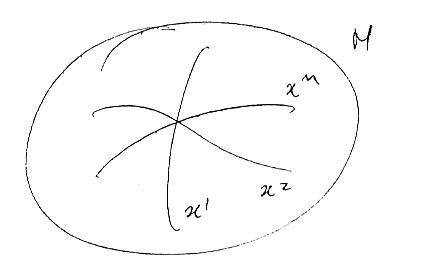
\includegraphics[width=0.75\columnwidth]{media/legame-tra-1-forma-di-poincare-cartan-e-dinamica/11-1.jpg}
  \end{minipage}
  \begin{minipage}[c]{.49\textwidth}
    $x^1,...,x^n$ coordinate locali su M\\
  \end{minipage}
\end{flushleft}

$ \eta = \eta_k (x^1, \dots , x^n) dx^k $ $ 1 $-forma differenziale su $ M $ \\
L'operazione di differenziazione, notoriamente definita nelle funzioni $ f : M \rightarrow \mathbb{R} $

\begin{equation} \label{eq:poin_cart_1}
  df = \frac{\partial f}{\partial x^k} \, (x^1, \dots , x^n) dx^k
\end{equation}

si estende nella $ 1 $-forma differenziale nel modo seguente

\begin{equation} \label{eq:poin_cart_2}
  d\eta = \frac{\partial \eta_{k}}{\partial x^r} \, dx^r \wedge dx^k = \frac{1}{2} \left( \frac{\partial \eta_{k}}{\partial x^r} - \frac{\partial \eta_{r}}{\partial x^k} \right) dx^r \otimes dx^k
\end{equation}

Osserviamo l'intrinsecità dell'operazione. Sia $ x'^k = x'^k (x^1, \dots , x^n) $ un cambiamento di coordinate

\begin{equation*}
  \begin{split}
    \eta &= \eta_k dx^k = \eta_k \frac{\partial x^k}{\partial x'^r} dx'^r \overset{def}{=} \eta'_r dx'^r\\
    &\Rightarrow \eta'_r=\eta_k \frac{\partial x^k}{\partial x'^r}
  \end{split}
\end{equation*}

Ora

\begin{equation*}
  \begin{split}
    & \left( \frac{\partial\eta'_k}{\partial x'^r} - \frac{\partial\eta'_r}{\partial x'^k} \right) dx'^r \otimes dx'^k = \\ 
    &= \left[ \frac{\partial}{\partial x'^r} \left( \eta_s \frac{\partial x^s}{\partial x'^k} \right) - \frac{\partial}{\partial x'^k} \left( \eta_s \frac{\partial x^s}{\partial x'^r} \right) \right] \frac{\partial x'^r}{\partial x^v} dx^v \otimes \frac{\partial x'^k}{\partial x^w} dx^w=\\
    &=\left[ \frac{\partial \eta_s}{\partial x'^r} \frac{\partial x^s}{\partial x'^k} + \cancel{\eta_s\frac{\partial ^2 x^s}{\partial x'^r\partial x'^k}} - \frac{\partial \eta_s}{\partial x'^k} \frac{\partial x^s}{\partial x'^r} + \cancel{\eta_s\frac{\partial ^2 x^s}{\partial x'^k\partial x'^r}} \right] \frac{\partial x'^r}{\partial x^v} dx^v \otimes \frac{\partial x'^k}{\partial x^w} dx^w=\\
    &= \left[ \frac{\partial x'^r}{\partial x^v} \frac{\partial \eta_s}{\partial x'^r} \frac{\partial x^s}{\partial x'^k} \frac{\partial x'^k}{\partial x^w} - \frac{\partial x'^k}{\partial x^w} \frac{\partial \eta_s}{\partial x'^k} \frac{\partial x^s}{\partial x'^r} \frac{\partial x'^r}{\partial x^v} \right] dx^v \otimes dx^w=\\
    &= \left[ \frac{\partial \eta_s}{\partial x^v} \delta^s w - \frac{\partial \eta_s}{\partial x^w} \delta^s v \right] dx^v \otimes dx^w = \\
    &= \left( \frac{\partial \eta_w}{\partial x^v} - \frac{\partial \eta_v}{\partial x^w} \right) dx^v \otimes dx^w
  \end{split}
\end{equation*}

e questo mostra che l'algoritmo di calcolo dato dalla ($ \ref{eq:poin_cart_2} $) è lo stesso in tutti i sistemi di ambiente, ovvero che l'operazione ($ \ref{eq:poin_cart_2} $) è intrinseca.\\
(Per esercizio provare che non è intrinseca l'operazione $ \frac{1}{2} \left( \frac{\partial \eta_{k}}{\partial x^r} + \frac{\partial \eta_{r}}{\partial x^k} \right) dx^r \otimes dx^k $).\\
In particolare, si osservi che, per un'arbitraria funzione $f$

\begin{equation*}
  \begin{split}
    ddf&=d \left( \frac{\partial f}{\partial x^k}dx^k\right) = \left( \frac{\partial}{\partial x^r} \frac{\partial f}{\partial x^k} - \frac{\partial}{\partial x^k} \frac{\partial f}{\partial x^r} \right) dx^r \otimes dx^k = 0
  \end{split}
\end{equation*}

\begin{flushright}
(vedi nota\footnote{Il termine $dF$ nella \textit{condizione di Lie} non influenza la dinamica ($ddF$ è autenticamente nullo)})
\end{flushright}

Applichiamo queste condizioni alla $ 1 $-forma differenziale di Poincaré-Cartan

\begin{equation*}
  \begin{split}
    \theta &= P_i dq^i - H (t, q^r, P_r) dt\\
    d\theta &= dP_i \wedge dq^i - \frac{\partial H}{\partial q^r} dq^r \wedge dt - \frac{\partial H}{\partial P_r} dP_r \wedge dt
  \end{split}
\end{equation*}

% INIZIO PAGINA 12

Ordinando gli elementi della base delle $ 1 $-forme differenziali nel modo seguente: $ \{ dt, dq^1, \dots , dq^n, dP_1, \dots , dP_n \} $, la matrice (antisimmetrica) rappresentabile dalla $ 2 $-forma differenziale $ d \theta $ è

\begin{equation*}
  \renewcommand\arraystretch{3}
  \begin{array}{c c}
    \qquad &
    \begin{array}{c c c}
      % \hphantom{\frac{\partial H}{\partial \uline{P}}} & \hphantom{\left( - \frac{\partial H}{\partial \uline{q}} \right)^T} & \hphantom{\left( - \frac{\partial H}{\partial \uline{P}} \right)^T}\\
      dt \qquad & d \uline{q} \qquad & d \uline{P} \qquad
    \end{array}\\
    \begin{array}{c}
      dt\\
      d \uline{q}\\
      d \uline{P}
    \end{array}&
    \begin{array}{| c | c | c |}
      \hline
      0 & \left( - \frac{\partial H}{\partial \uline{q}} \right)^T & \left( - \frac{\partial H}{\partial \uline{P}} \right)^T\\
      \hline
      \frac{\partial H}{\partial \uline{q}} & 0 & I_{n \times n}\\
      \hline
      \frac{\partial H}{\partial \uline{P}} & - I_{n \times n} & 0\\
      \hline
    \end{array}
  \end{array}_{(2n + 1) \times (2n + 1)}
\end{equation*}

Esiste uno ed un solo campo vettoriale $ Z $ (con componente $ 1 $ lungo $ \frac{\partial}{\partial t} $) che ``annulla'' la $ 2 $-forma differenziale $ d\theta $; esso è il campo tale che $ Z \rfloor d \theta = 0 $ e $ \langle Z, dt \rangle =1 $. Notare che $ d\theta $ è antisimmetrica e lo spazio ha dimensione dispari $ (2n+1) $; ma $ Z $ t.c. $ Z \rfloor d \theta = 0 $ esiste certamente, e la condizione $ \langle Z, dt \rangle = 1 $ lo ``normalizza''.\\

\begin{equation*}
  Z = \frac{\partial}{\partial t} + \frac{\partial H(t,q^r,P_r)}{\partial P_k} \frac{\partial}{\partial q^k} - \frac{\partial H(t,q^r,P_r)}{\partial q^k} \frac{\partial}{\partial P_k}
\end{equation*}

matematicamente equivalente al sistema hamiltoniano

\begin{equation*}
  \begin{split}
    \frac{dt}{dt} &= 1 \\
    \frac{dq^k}{dt} &= \frac{\partial H(t,q^r,P_r)}{\partial P_k} \\
    \frac{dP_k}{dt} &= - \frac{\partial H(t,q^r,P_r)}{\partial q^k} \\
  \end{split}
\end{equation*}

\begin{flushleft}
  \begin{minipage}[c]{.5\textwidth}
    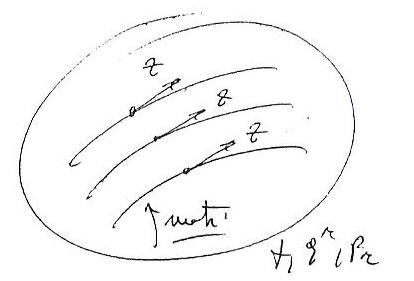
\includegraphics[width=0.75\columnwidth]{media/legame-tra-1-forma-di-poincare-cartan-e-dinamica/12-1.jpg}
  \end{minipage}
\end{flushleft}

\subsection{Dinamica di un sistema in termini della $ 1 $-forma differenziale di Poincaré-Cartan}

\begin{equation*}
\begin{split}
\text{\large$\theta$}_{\Lagr} &= \Lagr dt + \frac{\partial \Lagr}{\partial \dot{q}^k}\;\omega ^k = \Lagr dt + \frac{\partial \Lagr}{\partial \dot{q}^k}(dq^k-\dot{q}^k dt)= -\left(\frac{\partial \Lagr}{\partial \dot{q}^k} \dot{q}^k - \Lagr \right)dt + \frac{\partial \Lagr}{\partial \dot{q}^k} dq^k=\\ &= -H(t,q,\dot{q})dt + \frac{\partial \Lagr}{\partial \dot{q}^k} dq^k
\end{split}
\end{equation*}

\hspace*{-0.11 cm}$\text{\large$\theta$}_{\Lagr}$ è detta $ 1 $-forma di Poincaré-Cartan su $ j_1 (\mathcal{V}_{n+1}) $ associata alla Lagrangiana $ \Lagr $.

\begin{equation*}
\begin{split}
d\text{\large$\theta$}_{\Lagr} &= d\Lagr \wedge dt + d \left(\frac{\partial \Lagr}{\partial \dot{q}^k}\right) \wedge \omega ^k + \frac{\partial \Lagr}{\partial \dot{q}^k} d \omega ^k\\
&= d\Lagr \wedge dt + d \left(\frac{\partial \Lagr}{\partial \dot{q}^k}\right) \wedge \omega ^k - \frac{\partial \Lagr}{\partial \dot{q}^k} d \dot{q}^k \wedge dt\\
&= \frac{d \Lagr}{dq^k} dq^k \wedge dt + \cancel{\frac{\partial \Lagr}{\partial \dot{q}^k} d \dot{q}^k \wedge dt} + d \left(\frac{\partial \Lagr}{\partial \dot{q}^k}\right) \wedge \omega ^k - \cancel{\frac{\partial \Lagr}{\partial \dot{q}^k} d \dot{q}^k \wedge dt}\\
&= \frac{d \Lagr}{dq^k} dq^k \wedge dt + d \left(\frac{\partial \Lagr}{\partial \dot{q}^k}\right) \wedge \omega ^k\\
&= \frac{d \Lagr}{dq^k} \omega ^k \wedge dt + d \left(\frac{\partial \Lagr}{\partial \dot{q}^k}\right) \wedge \omega ^k
\end{split}
\end{equation*}

Posto $ Z = \frac{\partial}{\partial t} + y^i \frac{\partial}{\partial q^i} + Z^i \frac{\partial}{\partial \dot{q}^i} $ la condizione $ Z \rfloor \theta_{\Lagr} = 0 $ diventa

\begin{equation*}
\begin{split}
0 &= Z \rfloor \left[\frac{\partial \Lagr}{\partial q^k} \omega^k \wedge dt + d \left( \frac{\partial \Lagr}{\partial \dot{q}^k} \right) \wedge \omega^k \right]\\
&= \frac{\partial \Lagr}{\partial q^k} \left[ \left( Z \rfloor \omega^k \right) dt - \langle Z, dt\rangle \omega^k \right] + \langle Z, d \left( \frac{\partial \Lagr}{\partial \dot{q}^k} \right) \rangle \omega^k -d \left( \frac{\partial \Lagr}{\partial \dot{q}^k} \right) Z \rfloor \omega^k
\end{split}
\end{equation*}

ora $ Z \rfloor \omega^k = \langle Z, dq^k - \dot{q}^k dt \rangle = y^k - \dot{q}^k $, mentre $ \langle Z, dt \rangle = 1 $ per cui si ha:

% INIZIO PAGINA 13

\begin{equation*}
\begin{split}
0&=\frac{\partial \Lagr}{\partial \dot{q}^k}(y^k - \dot{q}^k)dt - \frac{\partial \Lagr}{\partial q^k}w^k + Z \left(\frac{\partial \Lagr}{\partial \dot{q}^k}\right) w^k - d\left(\frac{\partial \Lagr}{\partial \dot{q}^k}\right)(y^k - \dot{q}^k) \\
& =\left[ Z \left( \frac{\partial \Lagr}{\partial \dot{q}^k}\right) - \frac{\partial \Lagr}{\partial q^k} \right] w^k + \frac{\partial \Lagr}{\partial \dot{q}^k}(y^k - \dot{q}^k) dt - d \left( \frac{\partial \Lagr}{\partial \dot{q}^k}\right) (y^k - \dot{q}^k)
\end{split}
\end{equation*}

Sviluppando l'ultimo termine

\begin{equation*}
- d\left(\frac{\partial \Lagr}{\partial \dot{q}^k}\right)(y^k- \dot{q}^k) = - \left[\frac{\partial^2 \Lagr}{\partial t \partial \dot{q}^k}dt + \frac{\partial^2 \Lagr}{\partial q^r \partial \dot{q}^k}dq^r + \frac{\partial^2 \Lagr}{\partial \dot{q}^r \partial \dot{q}^k}d\dot{q}^r\right](y^k- \dot{q}^k)
\end{equation*}

si vede che esso è l'unico ad avere componenti lungo $d\dot{q}^r$ (si assuma, ad esempio, di usare la base $ \{dt, w^k=dq^k - \dot{q}^kdt, d\dot{q}^k\} $ per le forme differenziali su $j_1(\mathcal{V}_{n+1})$). \\
La condizione $Z \rfloor d \theta_{\Lagr} = 0$ implica pertanto che il termine $ - d \left(\frac{\partial \Lagr}{\partial \dot{q}^k}\right)(y^k - \dot{q}^k) $ debba essere nullo e, nell'ipotesi di non singolarità di $ \Lagr $ $ \left(\Leftrightarrow det \left( \frac{\partial^2 \Lagr}{\partial \dot{q}^r \partial \dot{q}^k}\right) \neq 0 \right)$ che $ y^k = \dot{q}^k $. \\
Pertanto la condizione $ Z \rfloor d \theta_{\Lagr} = 0 $ si riduce a
\begin{equation*}
\left(Z\left(\frac{\partial \Lagr}{\partial \dot{q}^k}\right)- \frac{\partial \Lagr}{\partial q^k}\right)w^k = 0
\end{equation*}
ovvero
\begin{align*}
&Z\left(\frac{\partial \Lagr}{\partial \dot{q}^k}\right)- \frac{\partial \Lagr}{\partial q^k} = 0	&k = 1, \dots , n
\end{align*}
\\ 
Risulta pertanto provato il fatto seguente: data $ \Lagr = \Lagr (t, q^r, \dot{q}^r) $ e definita la $ 1 $-forma di Poincaré-Cartan $ \theta_{\Lagr} $, le condizioni

\begin{equation*}
\begin{cases}
Z \rfloor d \theta_{\Lagr} = 0 \\
\langle Z,dt \rangle =1 \quad \Leftrightarrow \quad Z = \frac{\partial}{\partial t} + y^i \frac{\partial}{\partial q^i} + Z^i \frac{\partial}{\partial \dot{q}^i}\\
\end{cases}
\end{equation*}

determinano univocamente il campo vettoriale dinamico $ Z = \frac{\partial}{\partial t} + \dot{q}^i \frac{\partial}{\partial q^i} + Z^i (t, q, \dot{q}) \frac{\partial}{\partial \dot{q}^k} $ che \textit{geometrizza} le equazioni di Lagrange. \\
Quanto visto fino ad ora può essere riscritto in linguaggio Hamiltoniano. Detta

\begin{equation*}
\theta_H = P_i dq^i - H (t, q^k, P_k) dt
\end{equation*}

la $ 1 $-forma di Poincaré-Cartan associata all'Hamiltoniana $ H $, mostriamo che il campo vettoriale dello spazio tempo delle fasi che \textit{geometrizza} la meccanica Hamiltoniana

\begin{equation*}
Z = \frac{\partial}{\partial  t} + \frac{\partial H}{\partial P_i}\frac{\partial}{\partial q^i} - \frac{\partial H}{\partial q^i}\frac{\partial}{\partial P_i} \quad \Leftrightarrow \quad 
\begin{cases}
\frac{dq^i}{dt} = \frac{\partial H}{\partial P_i}\\
\frac{dP_i}{dt} = - \frac{\partial H}{\partial q^i}
\end{cases}
\end{equation*}

è esprimibile intrinsecamente attraverso le condizioni

\begin{equation*}
\begin{cases}
Z \rfloor d \theta_{H} = 0 \\
\langle Z,dt \rangle =1
\end{cases}
\end{equation*}

Osserviamo che la condizione $ \langle Z,dt \rangle =1 $ impone che la componente lungo $ \frac{\partial}{\partial t} $ sia uguale a $ 1 $. Partiamo perciò da un campo $ Z $ del tipo

\begin{equation*}
Z = \frac{\partial}{\partial  t} + Z^i\frac{\partial}{\partial q^i} + Z_i\frac{\partial}{\partial P_i}
\end{equation*}

e imponiamo la condizione $ Z \rfloor d \theta_{H} = 0 $

\begin{equation*}
\begin{split}
Z \rfloor d \theta_{H} &= \left( \frac{\partial}{\partial  t} + Z^i\frac{\partial}{\partial q^i} + Z_i\frac{\partial}{\partial P_i}\right) \rfloor (dP_k \wedge dq^k - dH(t, q^r, P_r) \wedge dt)\\
&= \left( \frac{\partial}{\partial  t} + Z^i\frac{\partial}{\partial q^i} + Z_i\frac{\partial}{\partial P_i}\right) \rfloor \left(dP_k \wedge dq^k - \frac{\partial H}{\partial q^k}dq^k \wedge dt - \frac{\partial H}{\partial P_k}dP_k \wedge dt \right)\\
&= \frac{\partial H}{\partial q^k}dq^k + \frac{\partial H}{\partial P_k}dP_k - Z^idP_i - Z^i \frac{\partial H}{\partial q^i}dt + Z_idq^i - Z_i\frac{\partial H}{\partial P_i}dt
\end{split}
\end{equation*}

per cui la condizione $ Z \rfloor d \theta_{H} = 0 $ implica

\begin{equation*}
Z_i = - \frac{\partial H}{\partial q^i} \qquad e \qquad Z^i = \frac{\partial H}{\partial P_i}
\end{equation*}

ovvero

\begin{equation*}
Z = \frac{\partial}{\partial  t} + \frac{\partial H}{\partial P_i}\frac{\partial}{\partial q^i} - \frac{\partial H}{\partial q^i}\frac{\partial}{\partial P_i}
\end{equation*}

% INIZIO PAGINA 14

Quanto visto precedentemente mostra che il campo dinamico $ Z $ \textit{più che dalla forma differenziale} $ \theta_H $ (o $ \theta_{\Lagr} $ in linguaggio lagrangiano) dipende \textit{dal suo differenziale} $ d \theta_H $ attraverso la condizione $ Z \rfloor d\theta_H = 0 $ (o da $ d\theta_{\Lagr} $ attraverso la condizione $ Z \rfloor d\theta_H = 0 $ in linguaggio lagrangiano). \footnote{Si potrebbe commentare questo fatto dicendo che $ \theta_H $ (o $ \theta_{\Lagr} $) è un ``potenziale'' per la dinamica.} \\
Risulta pertanto completamente motivata l'introduzione della \textit{``condizione di Lie''} su una trasformazione di coordinate $ t, q^k, P_k \rightarrow t, q'^k, P'^k $. Se una trasformazione soddisfa la condizione di Lie, la forma differenziale

\begin{equation*}
\theta = P_i dq^i - H (t, q^r, P_r) dt
\end{equation*}

si esprime nelle nuove coordinate, nella forma

\begin{equation*}
\theta = P'_i dq'^i - H (t, q^r, P_r) dt + dF
\end{equation*}

ma

\begin{equation*}
d\theta = d (P_i dq^i - H dt) + ddF
\end{equation*}
e $ddF=0$ \footnote{L'aggiunta di un differenziale al ``potenziale'' non cambia la dinamica} per ogni $ F $, e il campo dinamico $ Z $ determinato da

\begin{align*}
&Z \rfloor (dP_i \wedge dq^i - H \wedge dt) = 0
\\&\langle Z,dt\rangle = 1
\end{align*}

oppure da

\begin{align*}
&Z \rfloor (dP'_i \wedge dq'^i - H' \wedge dt) = 0
\\ &\langle Z,dt\rangle = 1
\end{align*}

hanno la stessa truttura (Hamiltoniana) rappresentativa:

\begin{equation*}
Z= \frac{\de}{\de t}+\frac{\de H}{\de P_i} \frac{\de}{\de q^i}- \frac{\de H}{\de q^i} \frac{\de}{\de P_i} = \frac{\de}{\de t'} + \frac{\de H'}{\de P'_i} \frac{\de}{\de q'^i} - \frac{\de H'}{\de q'^i} \frac{\de}{\de P'_i}
\end{equation*}
\section{Teoria di Hamilton-Jacobi}
\setcounter{equation}{0}

Abbiamo visto che una funzione $ F = F (t, q^i, q'^i) $ con la proprietà che

\begin{equation*}
det \left( \frac{\de^2 F}{\de q^i \de q'^k}\right) \neq 0
\end{equation*}

può giocare il ruolo di funzione generatrice di una trasformazione

\begin{equation}
t' = t \qquad q'^k = q'^k (t, q^r, P_r) \qquad P'_k = P'_k (t, q^r, P_r)
\end{equation}

che preserva la struttura di ogni sistema Hamiltoniano. Precisamente, dalla condizione di Lie abbiamo che \\

\begin{subnumcases}{}
P_i= \frac{\de F (t,q^k,q'^k)}{\de q^i} \label{eq:ham_jac_2a}\\
P'_i= - \frac{\de F (t,q^k,q'^k)}{\de q'^i} & i=1,\dots ,n\\
H'= H + \frac{\de F (t,q^k,q'^k)}{\de t} \label{eq:ham_jac_2c}
\end{subnumcases}

e abbiamo visto che una trasformazione che soddisfa la condizione di Lie ha jacobiano $ M = M (t, q^r, P_r) $ che soddisfa $ M^T J M = J $. Di conseguenza una trasformazione che soddisfa la condizione di Lie preserva la struttura di ogni sistema Hamiltoniano.\\
Nel seguito chiameremo \textit{canoniche} queste trasformazioni. \\

% FINE PAGINA 14 - INIZIO PAGINA 15

Il carattere \textit{non invariante} di $ H $ rispetto a trasformazioni canoniche (come risulta esplicitamente dalla ($ \ref{eq:ham_jac_2c} $)) può essere utilmente sfruttato, e precisamente è possibile porsi il problema di determinare una opportuna trasformazione canonica, generata da un'opportuna funzione generatrice $ F = F (t, q^k, q'^k) $, tale che la ``nuova'' Hamiltoniana $ H' = H' (t, q'^k, P'_k) $ risulti \textit{identicamente nulla}. \\
Essendo la trasformazione canonica, la struttura Hamiltoniana del sistema verrà preservata e precisamente il sistema:

\begin{equation*}
\begin{cases}
\frac{dq^k}{dt}= \frac{\de H (t, q^r, P_r)}{\de P_k}\\
\frac{dP_k}{dt}= - \frac{\de H (t, q^r, P_r)}{\de q^k}
\end{cases}
k=1, \dots , n
\end{equation*}

dopo aver subito la trasformazione

\begin{equation*}
t' = t, \quad q'^k = q'^k (t, q^r, P_r), \quad P'_k = P'_k (t, q^r, P_r)
\end{equation*}

si potrà riscrivere ancora nella forma

\begin{equation*}
\begin{cases}
\frac{dq'^k}{dt}= \frac{\de H' (t, q'^r, P'_r)}{\de P'_k}\\
\frac{dP'_k}{dt}= - \frac{\de H' (t, q'^r, P'_r)}{\de q'^k}
\end{cases}
k = 1, \dots , n
\end{equation*}

Ora, se $ H' = H' (t, q'^r, P'_r) = 0 $

\begin{equation*}
\begin{cases}
\frac{dq'^k}{dt}= \frac{\de H'}{\de P'_k} = 0\\
\frac{dP'_k}{dt}= - \frac{\de H'}{\de q'^k} = 0
\end{cases}
k = 1, \dots , n
\end{equation*}

Pertanto, nelle variabili $ q'^k, P'_k $ ogni moto del sistema avrà una descrizione banale, e precisamente

\begin{align*}
q'^k (t) & = q'^k_0 \\
P'_k (t) & = {P'_k}_0
\end{align*}

le quantità $ q'^k_0 $ e $ {P'_k}_0 $ dipendono dai $ 2n $ dati iniziali del problema.\\
La soluzione del problema del moto è pertanto ricondotta alla determinazione del legame tra le variabili $ q'^k, P'_k $ e le variabili $ q^k, P_k $, ovvero alla trasformazione

\begin{eqnarray*}
q^k &= q^k(t,q'^k,P'_k) = q^k(t,q'^k_0,{P'_k}_0)\\
P_k &= P_k(t,q'^k,P'_k) = P_k(t,q'^k_0,{P'_k}_0)
\end{eqnarray*}

La condizione che determina la $F=F(t,q^k,q'^k)$ tale che $H'(t,q'^k,P'_k)=0$ è, per la ($ \ref{eq:ham_jac_2c} $)

\begin{equation*}
0=H \left( t,q^k,P_k(t,q^r,q'^r) \right) + \frac{\de F(t,q^r,q'^r)}{\de t}
\end{equation*}

ovvero, per la ($ \ref{eq:ham_jac_2a} $)

\begin{equation} \label{eq:ham_jac_3}
0=H \left( t,q'^k,\frac{\de F(t,q^r,q'^r)}{\de q^k} \right) + \frac{\de F(t,q^r,q'^r)}{\de t}
\end{equation}

\begin{footnotesize}
[Notare che si sono usate le coordinate $t,q^r,q'^r$, trattate come indipendenti, per esprimere tutte le quantità che compaiono nella relazione ($ \ref{eq:ham_jac_2c} $)].
\end{footnotesize}
\\

L'equazione ($ \ref{eq:ham_jac_3} $) ha la natura di un'equazione alle derivate parziali del primo ordine, in cui

\begin{enumerate}
\item[] $t,q^k$ sono le variabili indipendenti
\item[] $F$ è la funzione incognita
\item[] $q'^k$ intervengono nella ($ \ref{eq:ham_jac_3} $) parametricamente
\end{enumerate}

Il ruolo dei parametri $q'^k$ sarà ben spiegato nelle righe seguenti.\\

% INIZIO PAGINA 16

Come già detto l'equazione

\begin{equation} \label{eq:ham_jac_4}
H \left( t,q^k,\frac{\de F}{\de q^k} \right) + \frac{\de F}{\de t}=0
\end{equation}

è alle derivate parziali del primo ordine, $ t, q^k $ sono variabili indipendenti e $ F $ la funzione incognita. Nessun dato ``al bordo'' è significativo, per cui la ($ \ref{eq:ham_jac_4} $) ha infinite soluzioni.

Per i nostri scopi,  ovvero per costruire un trasformazione, della ($ \ref{eq:ham_jac_4} $) non basta però determinare una soluzione, ma occorre determinare una famiglia di soluzioni, parametrizzate dalle $n$ variabili $q'^k$ (Precisamente, ogni assegnazione della $n$-upla $q'^1,\dots,q'^n$ individua una soluzione della ($ \ref{eq:ham_jac_4} $)).\\
Occorre che la dipendenza delle soluzioni della ($ \ref{eq:ham_jac_4} $) dai parametri $q'^n$ sia ``significativa'', ovvero che

\begin{equation} \label{eq:ham_jac_5}
det \left( \frac{\de^2 F}{\de q'^k \de q^i}\right) \neq 0
\end{equation}

Una famiglia di soluzioni $F(t,q^k,q'^1,\dots,q'^n)$ della ($ \ref{eq:ham_jac_4} $) è quello che nel gergo viene detto un \textit{integrale completo}, ovviamente quando la ($ \ref{eq:ham_jac_5} $) è soddisfatta. Noto un integrale completo della ($ \ref{eq:ham_jac_4} $) è possibile costruire la trasformazione  canonica che banalizza il sistema Hamiltoniano.
\section{Esercizi sulla teoria di Hamilton-Jacobi}
\setcounter{equation}{0}

Considerata la funzione generatrice $ F $ nella forma:

\begin{equation*}
F = F (t, q^k, q'^k)
\end{equation*}

la trasformazione tra le varibili $ t, q^k, P_k $ e $ t' = t, q'^k, P'_k $ è data, in moto involuto, da

\begin{subequations}{\label{eq:es_ham_jac_1}}
\begin{eqnarray}
P_i = \frac{\de F (t, q^k, q'^k)}{\de q^i}\\ \label{eq:es_ham_jac_1a}
P'_i = - \frac{\de F (t, q^k, q'^k)}{\de q'^i} \label{eq:es_ham_jac_1b}
\end{eqnarray}
\end{subequations}

e l'equazione di Hamilton-Jacobi prende la forma

\begin{equation}
H \left(t, q^k, \frac{\de F}{\de q^k} \right) + \frac{\de F}{\de t} = 0
\end{equation}


%\hline QUI BISOGNA INSERIRE UNA LINEA


\subsubsection*{Oscillatore armonico}

\begin{equation}
H = H (t, q, P)= \frac{P^2}{2m} + \frac{1}{2} m \omega^2q^2
\end{equation}

Cerco $F$ nella forma

\begin{equation}
F = F (t, q, q') = - q' t + w (q, q')
\end{equation}

\begin{equation}
\frac{1}{2m} {\left( \frac{\de w}{\de q} \right)}^2+\frac{1}{2} m \omega^2q^2=q'
\end{equation}

Notare che il parametro $ q' $ si identifica con l'energia totale, per cui lo indicheremo con $ h $.

\begin{align*}
\frac{\de w}{\de q} &= \sqrt{m} \sqrt{2h - m \omega^2q^2}\\
w (q, h) &= \int \sqrt{m} \sqrt{2h - m \omega^2q^2} dq~(+ c)
\end{align*}

\begin{equation}
F (t, q, h) = - h t + \sqrt{m} \int \sqrt{2h + m \omega^2 q^2} dq ~ (+ c)
\end{equation}

per la ($ \ref{eq:es_ham_jac_1} a, b $) la trasformazione di coordinate fornita da $ F (t, q, q') $, dove $ q' = h $ è perciò

\begin{align*}
P &= \frac{\partial F (t, q, h)}{\partial q} \\
P' &= -\frac{\partial F (t, q, h)}{\partial h}
\end{align*}

\begin{equation*}
\begin{split}
P' &= - \frac{\partial F}{\partial h} = t - \frac{\partial w}{\partial h} = t - \sqrt{m} \mathlarger{\int{\frac{dq}{\sqrt{2h - m \omega^2 q^2}}}} \\
&= t - \frac{1}{\omega} \mathlarger{\int{\frac{dq}{\sqrt{\frac{2h}{m\omega^2} - q^2}}}} = t - \frac{1}{\omega} arcsin \left( \sqrt{\frac{m \omega^2}{2h}} q \right)
\end{split}
\end{equation*}

Che, risolta rispetto a $ q $, fornisce

\begin{equation*}
\omega (t - P') = arcsin \left( \sqrt{\frac{m\omega^2}{2h}} q \right)
\end{equation*}

\begin{equation} \label{eq:es_ham_jac_7}
q (t, q', P') = \sqrt{\frac{2h}{m \omega^2}} sin(\omega(t - P'))
\end{equation}

che fornisce $ q $ in funzione del tempo e delle $ 2 $ quantità costanti lungo ogni moto

\begin{align*}
&q' = h = (\text{energia totale}) \\
&P' \qquad \quad (\text{fase temporale})
\end{align*}

Per completezza abbiamo

\begin{equation} \label{eq:es_ham_jac_8}
P = \frac{\partial F}{\partial q} = \frac{\partial w}{\partial q} = \sqrt{m} \sqrt{2h - m \omega^2 q^2}
\end{equation}

e sostituendo in ($ \ref{eq:es_ham_jac_8} $) quanto ricavato nella ($ \ref{eq:es_ham_jac_7} $), abbiamo $P = P (t, q', P')$ ovvero $P$ in funzione del tempo e delle due quantità conservate $q' = h$, $P'$.

\subsubsection*{Campo centrale}

\begin{equation}
H = H (t, r, \theta, P_r, P_\theta) = \frac{P_r^2}{2m} + \frac{P_\theta^2}{2mr^2} + V(r)
\end{equation}

Cerco $ F $ nella forma

\begin{equation*}
 F = F (t, r, \theta, q'^1, q'^2) = - q'^1 t + w (r, \theta, q'^1, q'^2)
\end{equation*}

l'equazione di Hamilton-Jacobi diventa

\begin{equation*}
\frac{1}{2m} \left( \frac{\partial w}{\partial r} \right)^2 + \frac{1}{2mr^2} \left( \frac{\partial w}{\partial \theta} \right)^2 + V(r) = q'^1 \qquad q'^1~energia~totale
\end{equation*}

Cerchiamo $ w (r, \theta, q'^1, q'^2) $ nella forma

\begin{equation*}
\begin{split}
& w = w (r, \theta, q'^1, q'^2) = w_r(r, q'^1, q'^2) + w_\theta(\theta, q'^1, q'^2) \\
& \left[ \frac{1}{2m} \left( \frac{\partial w_r}{\partial r} \right)^2 + V(r) - q'^1 \right] 2mr^2 = -\left( \frac{\partial w_\theta}{\partial \theta} \right)^2 \\
& \begin{cases}\left[ \frac{1}{2m} \left( \frac{\partial w_r}{\partial r} \right)^2 + V(r) - q'^1 \right] 2mr^2 = -\left( q'^2 \right)^2 \\
\left( \frac{\partial w_\theta}{\partial \theta} \right)^2 =  \left( q'^2 \right)^2
\end{cases}
\end{split}
\end{equation*}

essendo $ q'^2 $ una unica quantità costante lungo ogni moto, che si identifica col momento della quantità di moto del sistema.

\begin{equation*}
\begin{split}
& w_r (r, q'^1, q'^2) = \mathlarger{\int} \sqrt{2m q'^1 - 2m V(r) -\frac{\left( q'^2 \right)^2}{r^2}} dr \\
& w_\theta (\theta, q'^1, q'^2) = q'^2 \theta
\end{split}
\end{equation*}

\begin{align*}
F (t, r, \theta, q'^1, q'^2) &= - q'^1 t + w (r, \theta, q'^1, q'^2) = - q'^1 t + q'^2 \theta +
\\
&+ \mathlarger{\int} \sqrt{2m q'^1 - 2m V(r) - \frac{\left( q'^2 \right)^2}{r^2}} dr
\end{align*}

La trasformazione è data da

\begin{align*}
& P_r = \frac{\partial F}{\partial r} & P_\theta = \frac{\partial F}{\partial \theta}
\\
& P'_1 = \frac{\partial F}{\partial q'^1} & P'_2 = \frac{\partial F}{\partial q'^2}
\end{align*}

\begin{equation*}
\begin{split}
& P'_1 = - \frac{\partial F}{\partial q'^1} = t - \mathlarger{\int} \frac{2m}{2 \sqrt{2m q'^1 - 2m V(r) - \frac{\left( q'^2 \right)^2}{r^2}}}dr \\
& P'_2 = - \frac{\partial F}{\partial q'^2} = \theta - \mathlarger{\int} \frac{ \frac{- 2 q'^2}{r^2} }{2 \sqrt{2m q'^1 - 2m V(r) - \frac{\left( q'^2 \right)^2}{r^2}}}dr
\end{split}
\end{equation*}


\section{Un po' più di geometria (simplettica)}
\setcounter{equation}{0}
Riepilogo della formulazione lagrangiana della meccanica classica \\

\begin{center}
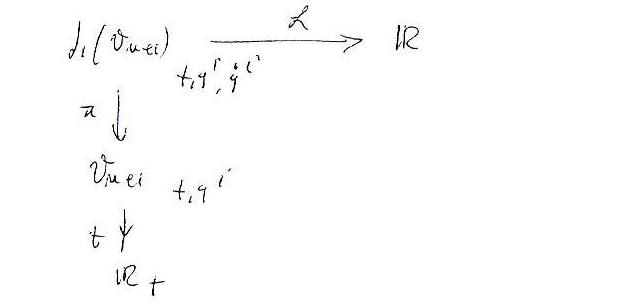
\includegraphics[width=0.5\columnwidth]{media/un-po-di-geometria-simplettica/18-1.jpg}
\end{center}

$ t, q^i $ coordinate fibrate su $\mathcal{V}_{n+1}$, spazio tempo degli eventi in presenza di vincoli \\

$ t, q^i, \dot{q}^i $ coordinate naturali in $j_1 (\mathcal{V}_{n+1})$, spazio tempo degli stati cinetici in presenza di vincoli. \\

\begin{equation*}
\begin{cases}
t' = t \\
q'^i = q'^i (t, q)
\end{cases}
\end{equation*}

\begin{center}
gruppo di trasformazione di coordinate in $\mathcal{V}_{n+1}$
\end{center}

\begin{equation*}
\begin{cases}
t' = t \\
q'^i = q'^i (t, q) \\
\dot{q}'^i = \frac{\partial q'^i}{\partial t} (t, q) + \frac{\partial q'^i}{\partial q^k} (t, q) \dot{q}^k
\end{cases}
\end{equation*}

\begin{center}
gruppo di trasfomazioni tra coordinate naturali di $j_1 (\mathcal{V}_{n+1})$
\end{center}

\begin{equation*}
\frac{d}{dt} \frac{\partial \Lagr}{\partial \dot{q}^k} - \frac{\partial \Lagr}{\partial q^k}
\end{equation*}

equazioni di Lagrange \\

\begin{align*}
&\Rightarrow \ddot{q}^k = \ddot{q}^k (t, q, \dot{q}) \overset{\underset{\mathrm{def}}{}}{=} Z^k (t, q, \dot{q}) \\
&\Rightarrow Z = \frac{\partial}{\partial t} + \dot{q}^k \frac{\partial}{\partial q^k} + Z^k (t, q, \dot{q}) \frac{\partial}{\partial \dot{q}^k}
\end{align*}

Nota: $ \Lagr' = \Lagr + \frac{d}{dt} f (t, q) $ e $ \Lagr $ determinano la stessa dinamica (gauge Lagrangiano). \\

\subsubsection*{Esercizio:}

\begin{align*}
\frac{\partial \Lagr}{\partial q^k} &= \frac{\partial \Lagr}{\partial q'^i} \frac{\partial q'^i}{\partial q^k} + \frac{\partial \Lagr}{\partial \dot{q}'^i} \frac{\partial \dot{q}'^i}{\partial q^k}
\\
\frac{\partial \Lagr}{\partial \dot{q}^k} &= \frac{\partial \Lagr}{\partial \dot{q}'^i} \frac{\partial \dot{q}'^i}{\partial \dot{q}^k} = \frac{\partial \Lagr}{\partial \dot{q}'^i} \frac{\partial q'^i}{\partial q^k}
\\
\frac{d}{dt} \frac{\partial \Lagr}{\partial \dot{q}^k} &= \left( \frac{d}{dt} \frac{\partial \Lagr}{\partial \dot{q}'^i} \right) \frac{\partial q'^i}{\partial q^k} + \frac{\partial \Lagr}{\partial \dot{q}'^i} \frac{d}{dt} \frac{\partial q'^i}{\partial q^k}
\\
&= \left( \frac{d}{dt} \frac{\partial \Lagr}{\partial \dot{q}'^i} \right) \frac{\partial q'^i}{\partial q^k} + \frac{\partial \Lagr}{\partial \dot{q}'^i} \frac{\partial \dot{q}'^i}{\partial q^k}
\end{align*}

\begin{equation*}
\Rightarrow \frac{d}{dt} \frac{\partial \Lagr}{\partial \dot{q}^k} - \frac{\partial \Lagr}{\partial q^k} = \left( \frac{d}{dt} \frac{\partial \Lagr}{\partial \dot{q}'^i} - \frac{\partial \Lagr}{\partial q'^i} \right) \frac{\partial q'^i}{\partial q^k}
\end{equation*}

Risulta pertanto mostrata l'invarianza delle equazioni di Lagrange al variare delle \textit{coordinate} in $\mathcal{V}_{n+1}$. \\

Posto $\omega^k = dq^k - \dot{q}^k dt$, un semplice calcolo mostra che

\begin{equation*}
\begin{split}
\omega'^i &= dq^k - \dot{q}'^i dt = \frac{\partial q'^i}{\partial q^k} (dq^k - \dot{q}^k dt) \\
&= \frac{\partial q'^i}{\de q^k} \omega^k
\end{split}
\end{equation*}

Pertanto le equazioni di Lagrange si possono scrivere in forma \textit{vettoriale} nel modo seguente:
\begin{equation*}
\sum_{k=1} ^{N} \left( \frac{d}{dt} \frac{\partial \Lagr}{\partial \dot{q}^k} - \frac{\partial \Lagr}{\partial q^k} \right) \omega^k = 0
\end{equation*}

Similmente, posto $\quad \mathcal{T}_{k|I} = \frac{d}{dt} \frac{\partial T_I}{\partial \dot{q}^k} - \frac{\partial T_I}{\partial q^k}\quad$ e $\quad Q_{k|I} = \sum_{i=1}^{N} F_{i|I} \cdot \frac{\partial P_i}{\partial q^k}$, si può scrivere:

\begin{equation*}
\sum_{k=1}^{N} \mathcal{T}_{k|I} \quad \omega ^k = \sum_{k=1}^{N} Q_{k|I} \quad \omega^k
\end{equation*}

% INIZIO PAGINA 19

\begin{equation*}
H = \frac{\partial \Lagr}{\partial \dot{q}^k}\dot{q}^k - \Lagr = \frac{\partial \Lagr}{\partial \dot{q}^i}\frac{\partial q'^i}{\partial q^k}\dot{q}^k - \Lagr
= \frac{\partial \Lagr}{\partial \dot{q}^i}\left(\dot{q}'^i - \frac{\partial q^i}{\partial t}\right) - \Lagr = H' - \frac{\partial \Lagr}{\partial \dot{q}^i}\frac{\partial q^i}{\partial t}
\end{equation*}

che mostra le leggi di trasformazione della \textit{funzione} Hamiltoniana al variare delle coordinate. \textit{Notare che} $H$ \textit{non è invariante per trasformazioni di coordinate restanti in} $j_1(\mathcal{V}_{n+1})$. \\

Osserviamo inoltre che

\begin{equation*}
\begin{aligned}
- H dt + \frac{\partial \Lagr}{\partial \dot{q}^k} q^k
&= - \left(H' - \frac{\partial \Lagr}{\partial \dot{q}^i}\frac{\partial q'^i}{\partial t}\right)dt + \frac{\partial \Lagr}{\partial \dot{q}^i}\frac{\partial q'^i}{\partial q^k} dq^k \\
&= -H'dt + \frac{\partial \Lagr}{\partial \dot{q}'^i} dq'^i
\end{aligned}
\end{equation*}

La quale mostra che la $ 1 $-forma differenziale, detta di Poincaré-Cartan,

\begin{equation*}
\theta_{\Lagr} = - H dt + \frac{\partial \Lagr}{\partial \dot{q}^k} dq^k
\end{equation*}

ha comportamento \textit{invariantivo} al cambiare delle coordinate. \\

Sotto una trasformazione di gauge $ \Lagr \rightarrow \Lagr' = \Lagr + \frac{df}{dt} $,

\begin{equation*}
\begin{aligned}
\theta_{\Lagr}
&= - H dt + \frac{\partial \Lagr}{\partial \dot{q}^k} dq^k = - \left (\frac{\partial \Lagr}{\partial \dot{q^k}}\dot{q^k} - \Lagr \right) dt + \frac{\partial \Lagr}{\partial \dot{q}^k} q^k \\
&= \Lagr dt + \frac{\partial \Lagr}{\partial \dot{q}^k} \left( dq^k - \dot{q^k} dt \right) = \Lagr dt + \frac{\partial \Lagr}{\partial \dot{q^k}}\omega^k
\end{aligned}
\end{equation*}
diventa
\begin{equation*}
\begin{aligned}
\theta'_{\Lagr} 
&= \left( \Lagr + \frac{df}{dt} \right) dt + \frac{\partial}{\partial \dot{q}^k} \left( \Lagr + \frac{df}{dt} \right) \left(dq^k - \dot{q^k} dt \right) \\
&= \Lagr dt + \frac{\partial f}{\partial t} dt + \frac{\partial \Lagr}{\partial \dot{q^k}}\omega^k + \frac{\partial f}{\partial q^k} \left(dq^k - \dot{q^k} dt\right) \\
&= \left( \Lagr dt + \frac{\partial \Lagr}{\partial \dot{q^k}}\omega^k \right) + \left( \frac{\partial f}{\partial t} dt + \cancel{\frac{\partial f}{\partial q^k} \dot{q^k}} \right) dt + \frac{\partial f}{\partial q^k} \left(dq^k - \cancel{\dot{q^k} dt}\right) \\
&= \theta_{\Lagr} + \frac{\partial f}{\partial t} dt + \frac{\partial f}{\partial q^k} dq^k = \theta_{\Lagr} + df
\end{aligned}
\end{equation*}

I calcoli come svolti mostrano che la $ 1 $-forma differenziale $ \theta_{\Lagr} = - H (t, q, \dot{q}) dt + \frac{\partial \Lagr}{\partial \dot{q^k}} (t, q, \dot{q}) dq^k $ sullo spazio $ j_1 (\mathcal{V}_{n+1}) $, detta $ 1 $-forma di Poincaré-Cartan associata a $ \Lagr $, è un oggetto importante. \\
La si incontrerà molte volte nelle pagine seguenti.

\section{Struttura simplettica del fibrato cotangente}
\setcounter{equation}{0}

Sia $M$ una varietà differenziabile (che poi identificheremo con $\mathcal{V}_{n+1}$) e che riferiremo per generalità e semplicità a coordinate locali $x^1, \dots , x^m$.
\begin{multicols}{2}
%\smallskip
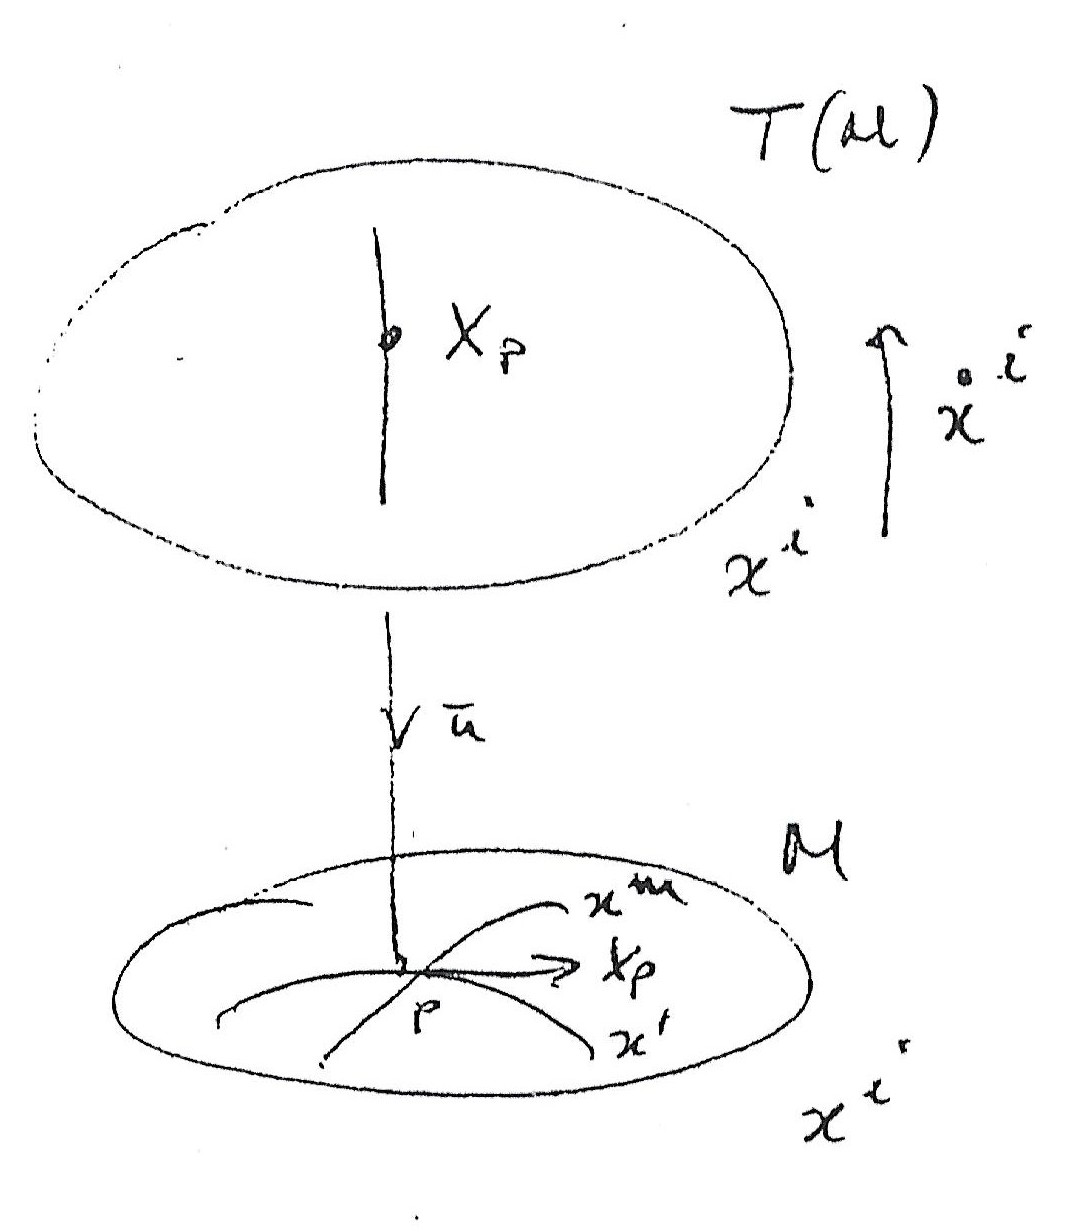
\includegraphics[width=\columnwidth]{media/struttura-simplettica-del-fibrato-cotangente/20-1}
\begin{equation*}
X_p = (X_P)^i \frac{\partial}{\partial x^i} \overset{def}{=} \dot{x}_P^i \bigg( \frac{\partial}{\partial x^i} \bigg)_P
\end{equation*}
$T(M) =$ spazio (fibrato su $M$) costituito dalla totalità dei \textit{vettori} applicati in tutti i punti di $M$
\\
$x^i, ~\dot{x}^i$ \quad coordinate \textit{naturali} su $T (M)$ \\
\begin{equation*}
X_P = \dot{x}_P^i \frac{\partial}{\partial x^i} = \dot{x}_P^i \frac{\partial x'^k}{\partial x^i}\frac{\partial}{\partial x'^k} 
\end{equation*}
\begin{equation*}
\left \{
\begin{aligned}
x'^i &= x'^i(x^1 \dots x^m) \\
\dot{x}'^i &= \frac{\partial x'^i}{\partial x^k} (x^1 \dots x^m) \dot{x}^k \\ 
\end{aligned}
\right.
\end{equation*}

\textit{Trasformazione} tra coordinate \textit{naturali} in $T (M)$ \\

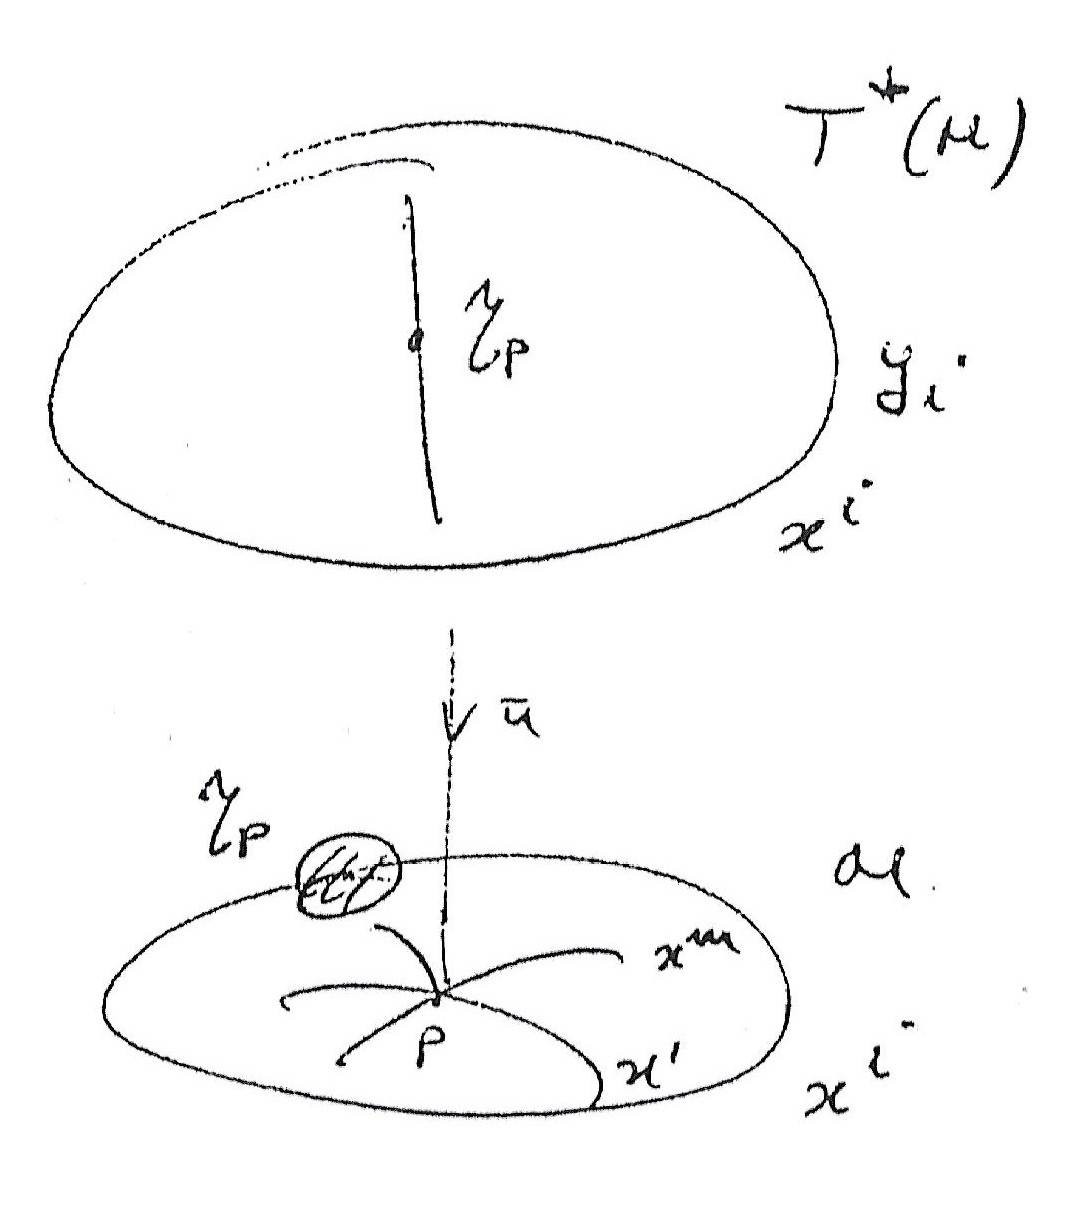
\includegraphics[width=\columnwidth]{media/struttura-simplettica-del-fibrato-cotangente/20-2}
\smallskip
\begin{equation*}
\eta_P = (\eta_P)_i dx^i \overset{def}{=} y_{i_p}(dx^i)_P 
\end{equation*}
\\
$T^*(M) =$ spazio (fibrato su $M$) costituito dalla totalità delle \textit{forme differenziali} applicate in tutti i punti di $M$ \\
$x^i, y_i$ \quad coordinate \textit{naturali} su $T^*(M)$ \\
\begin{equation*}
\eta_P = y_{i_P} dx^i = y_{i_P} \frac{\partial x'}{\partial x'^k} dx'^k 
\end{equation*}
\begin{equation*}
\left\{
\begin{aligned}
x'^i &= x'^i(x^1 \dots x^m) \\
y'^i &= \frac{\partial x^k}{\partial x'^i} (x^1 \dots x^m) y_k \\ 
\end{aligned}
\right.
\end{equation*}
\textit{Trasformazione} tra coordinate \textit{naturali} in $T^* (M)$ \\
\end{multicols}

Concentriamo la nostra attenzione su $ T^* (M) $. Esso ammette i seguenti oggetti invarianti o canonici

\begin{equation*}
\begin{aligned}
\theta &= y_i dx^i &\text{$ 1 $-\textit{forma di Liouville} su } T^* (M) \\
\Omega &= d\theta = dy_i \wedge dx^i &\text{$ 2 $-\textit{forma simplettica} su } T^* (M).
\end{aligned}
\end{equation*}

Per ogni coppia di valori

\begin{equation*}
\begin{aligned}
X &= X^i \frac{\partial}{\partial x^i} + X_i \frac{\partial}{\partial y_i} &\in T (T^* (M)) \\
Y &= Y^i \frac{\partial}{\partial x^i} + Y_i \frac{\partial}{\partial y_i} &\in T (T^* (M))
\end{aligned}
\end{equation*}
l'insieme di $ \Omega $ sulla coppia $ (X, Y) $ è definito da
\begin{equation*}
\Omega(X, Y) = X_i Y^i - X^i Y_i = 
\begin{pmatrix} X^i & X_i \end{pmatrix}
\begin{pmatrix} 0 & -I  \\  I & 0 \end{pmatrix}
\begin{pmatrix} Y^i \\ Y_i \end{pmatrix}
\end{equation*}

dove $ I = \begin{pmatrix} 1 & 0 & \dots \\ 0 & 1 & & \\  \vdots & & \ddots &  \end{pmatrix}_{m \times m}$ \medskip

Si dimostra facilmente, sulla base della legge di trasformazione tra coordinate naturali in $ T^*(M) $ dedotta a pagina precedente, e sulla legge di trasformazione da essa indotta sulle componenti $ X'^i, X'_i, Y'^i, Y'_i $, che $ \Omega (X, Y) \in \mathbb{R} $ risulta \textit{indipendente} dalla scelta delle coordinate, cioè che, introdotte componenti $ X^i, X_i, Y^i, Y_i $ e $ X'^i, X'_i, Y'^i, Y'_i $ dei valori $ X, Y $ nelle diverse coordinate naturali su $ T^* (M) $ si ha che

\begin{equation*}
X'_i Y'^i - X'^i Y'_i = X_i Y^i - X^i Y_i
\end{equation*}

(vedi pagina \pageref{pag:7b_fibr_cot}). \\

% INIZIO PAGINA 21

Il funzionale bilineare $ \Omega(\cdot,\cdot) $ \label{pag:7_fibr_cot} definisce un prodotto scalare (antisimmetrico), e quindi stabilisce una identificazione tra \textit{vettori} (= vettori \textit{controvarianti}) e \textit{forme differenziali} (= vettori \textit{covarianti}) definiti su $T^* (M)$. \\

Posto $ \omega = a_idx^i + b^idy_i \quad \in T^*(T^*(M)) $, il vettore ad esso associato risulta essere

\begin{equation*}
X_\omega = - b^i\frac{\partial}{\partial x^i} + a_i \frac{\partial}{\partial y_i} \quad \in T (T^* (M))
\end{equation*}

come facilmente si può verificare dalla definizione

\begin{equation*}
\langle \omega, Y \rangle = \Omega (X_\omega, Y) \qquad \forall \, Y \in T (T^* (M))
\end{equation*}

\newpage

\begin{multicols}{2}
%\begin{wrapfloat}{figure}{l}{0pt}
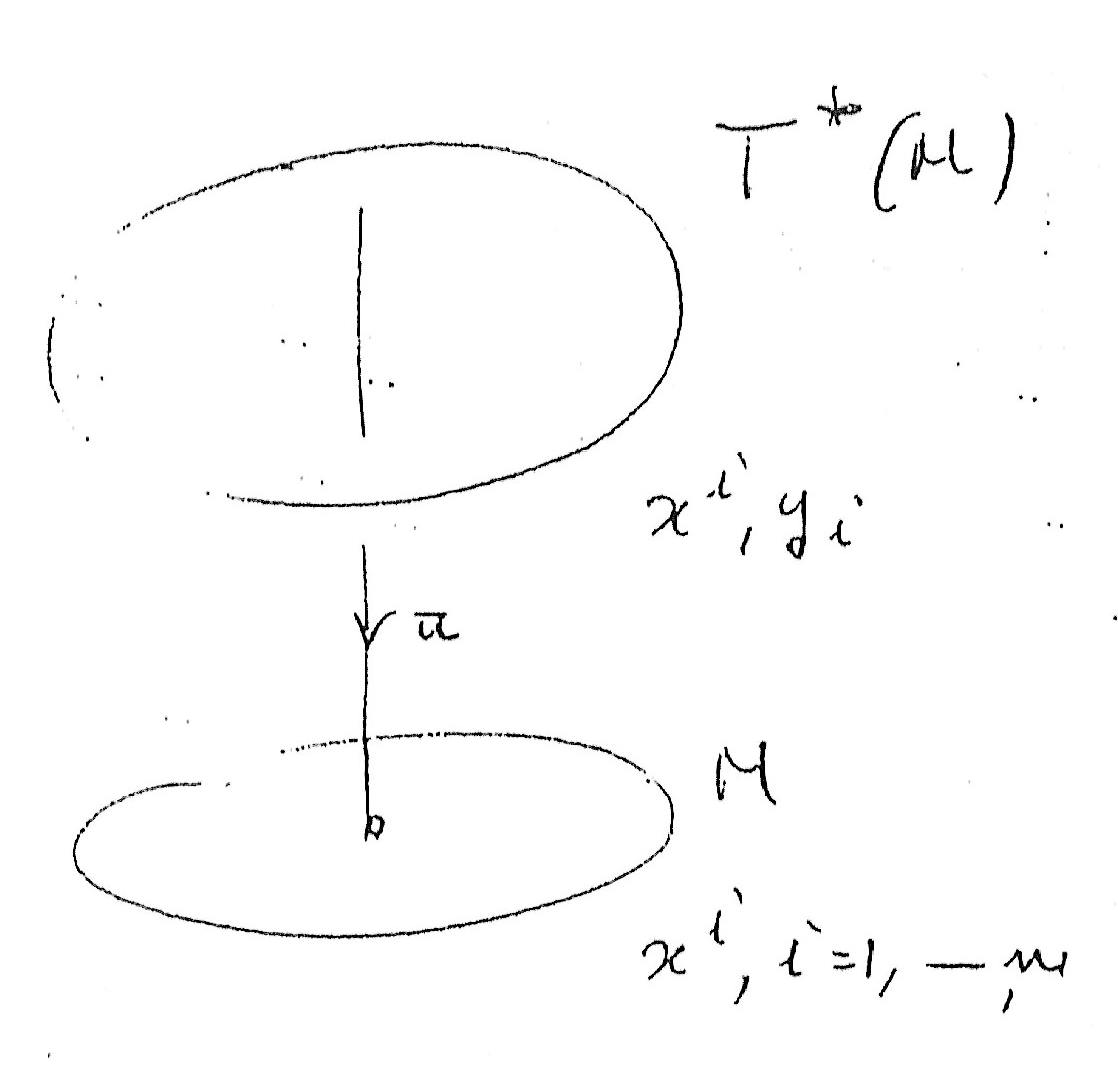
\includegraphics[width=\columnwidth]{media/struttura-simplettica-del-fibrato-cotangente/21-1.jpeg}
%\caption{Esempio di figura ‘‘avvolta’’ da un testo.}
%\end{wrapfloat}
\bigskip
\bigskip
\begin{equation*}
\eta_p \in T_p^* (M) \qquad \eta_p = y_i (dx^i)_p 
\end{equation*}
$ x^i, y_i $ coordinate \textit{``naturali''} in $T^*(M)$
\end{multicols}

Trasformazione tra coordinate naturali $ (x^i, y_i) \rightarrow (x'^i, y'_i) $ in $ T^* (M) $: 
\begin{equation*}
\left \{
\begin{aligned}
&x'^i = x'^i(x^1, \dots x^m) \quad \Leftrightarrow \quad x^k = x^k(x'^1, \dots x'^m) \\
&y'_i = \frac{\partial x^k}{\partial x'^i} (x^1, \dots x^m)y_k 
\end{aligned}
\right.
\end{equation*}

Sia $ X $ un campo vettoriale definito su $ T^* (M) $

\begin{equation*}
X = X^i \frac{\partial}{\partial x^i} + X_i\frac{\partial}{\partial y_i}
\end{equation*}

\begin{equation*}
\begin{aligned}
X &= X^i \bigg( \frac{\partial x'^k}{\partial x^i}\frac{\partial}{\partial x'^k} + \frac{\partial y'_k}{\partial x^i}\frac{\partial}{\partial y'_k} \bigg) + X_i \bigg( \frac{\partial x'^k}{\partial y_i}\frac{\partial}{\partial x'^k} + \frac{\partial y'_k}{\partial y_i}\frac{\partial}{\partial y'_k} \bigg) \\
&= X^i \frac{\partial x'^k}{\partial x^i}\frac{\partial}{\partial x'^k} + X^i \frac{\partial}{\partial x^i} \bigg( \frac{\partial x^r(x')}{\partial x'^k}y_r \bigg) \frac{\partial}{\partial y'_k} + X_i\frac{\partial x^i(x')}{\partial x'^k}\frac{\partial}{\partial y'_k} \\
&= X^i \frac{\partial x'^k}{\partial x^i}\frac{\partial}{\partial x'^k} + X^i \frac{\partial x'^s}{\partial x^i}\frac{\partial}{\partial x'^s} \frac{\partial x^r(x')}{\partial x'^k}y_r\frac{\partial}{\partial y'_k} + X_i\frac{\partial x^i(x')}{\partial x'^k}\frac{\partial}{\partial y'_k} \\
&= X^i \frac{\partial x'^k}{\partial x^i}\frac{\partial}{\partial x'^k} + \bigg( X^i \frac{\partial x'^s}{\partial x^i}\frac{\partial}{\partial x'^s} \frac{\partial x^r(x')}{\partial x'^k}y_r + X_i\frac{\partial x^i(x')}{\partial x'^k} \bigg) \frac{\partial}{\partial y'_k} \\
&\overset{def}{=} X'^k\frac{\partial}{\partial x'^k} + X'_k\frac{\partial}{\partial y'_k}
\end{aligned}
\end{equation*}

con

% INIZIO PAGINA 22

\begin{equation} \label{eq:strutt_fibr_cot_1}
\left\{
\begin{aligned}
X'^k &=: X^i \frac{\partial x'^k}{\partial x^i} \\
X'_k &=: X^i \frac{\partial x'^s}{\partial x^i}\frac{\partial}{\partial x'^s} \frac{\partial x^r(x')}{\partial x'^k}y_r + X_i\frac{\partial x^i(x')}{\partial x'^k}
\end{aligned}
\right.
\end{equation}

Riepilogando, sia $ (x^i, y_i) $ un sistema di coordinate \textit{naturali} su $T^*(M)$, e sia $ (x'^i, y'_i) $ un altro sistema di coordinate \textit{naturali}. Un campo vettoriale $X$ su $T^*(M)$ sarà rappresentato equivalentemente nella forma:
\begin{equation*}
X = X^i \frac{\partial}{\partial x^i} + X_i\frac{\partial}{\partial y_i} = X'^i\frac{\partial}{\partial x'^i} + X'_i\frac{\partial}{\partial y'_i}
\end{equation*}
e il legame tra le componenti $(X^i,X_i)$ e $(X'^i,X'_i)$ nei due sistemi di coordinate è dato dalla formula ($ \ref{eq:strutt_fibr_cot_1} $).\\
Consideriamo ora due campi
\begin{equation*}
\left.X=~\bigg\langle~
\begin{aligned} 
&X^i \frac{\partial}{\partial x^i} + X_i\frac{\partial}{\partial y_i} \\
&X'^i\frac{\partial}{\partial x'^i} + X'_i\frac{\partial}{\partial y'_i}
\end{aligned}
\qquad
\right.Y=~\bigg\langle~
\begin{aligned} 
&Y^i \frac{\partial}{\partial x^i} + Y_i\frac{\partial}{\partial y_i} \\
&Y'^i\frac{\partial}{\partial x'^i} + Y'_i\frac{\partial}{\partial y'_i}
\end{aligned}
\end{equation*}
e il funzionale bilineare (antisimmetrico) definito in coordinate naturali da:
\begin{equation*}
\Omega(X,Y) = X_kY^k - X^kY_k
\end{equation*} 
Mostriamo che la definizione sopra data è \textit{intrinseca}, cioè non dipende dalla scelta delle coordinate, ovvero notiamo che \label{pag:7b_fibr_cot}
\begin{equation*}
X'_kY'^k - X'^kY'_k = X_kY^k - X^kY_k
\end{equation*}
in ogni sistema di coordinate naturali.
\begin{equation*}
\begin{split}
X'_k Y'^k - X'^k Y'_k &= \\
&= \bigg( X^i \frac{\partial x'^s(x)}{\partial x^i}\frac{\partial^2 x^r(x')}{\partial x'^s \partial x'k}y_r + X^i \frac{\partial x^i(x')}{\partial x'^k} \bigg) Y^j\frac{\partial x'^k(x)}{\partial x^j} + \\ 
&\quad - X^i\frac{\partial x'^k(x)}{\partial x^i} \bigg(Y^j \frac{\partial x'^s(x)}{\partial x^i}\frac{\partial^2 x^r(x')}{\partial x'^s \partial x'k}y_r + X^i \frac{\partial x^i(x')}{\partial x'^k} \bigg) \\
&= X^i Y^j \frac{\partial x'^k(x)}{\partial x^j}\frac{\partial^2 x^r(x')}{\partial x'^s \partial x'k}\frac{\partial x'^s(x)}{\partial x^i}y_r + X_i Y^j \frac{\partial x^i(x')}{\partial x'^k}\frac{\partial x'^k(x)}{\partial x^j} + \\ 
&\quad - X^iY^j \frac{\partial x'^k(x)}{\partial x^i}\frac{\partial^2 x^r(x')}{\partial x'^s \partial x'k}\frac{\partial x'^s(x)}{\partial x^i}y_r - X^i Y_j \frac{\partial x'^k(x)}{\partial x^i}\frac{\partial x^j(x')}{\partial x'^k} \\
&= X^i Y^j \frac{\partial x'^s(x)}{\partial x^i}y_r + X_i Y^j - X^i Y^j \frac{\partial x'^s(x)}{\partial x^i}y_r - X^i Y_j \\
&= X_i Y^j - X^i Y_j
\end{split}
\end{equation*}

\section{Parentesi di Poisson in $T^* (M)$}
\setcounter{equation}{0}

Sia $ f : T^* (M) \rightarrow \mathbb{R} $ e

\begin{equation}
X_{df} = \frac{\partial f}{\partial x^i} \frac{\partial}{\partial y_j} -\frac{\partial f}{\partial y_j} \frac{\partial}{\partial x^i}
\end{equation}

il campo vettoriale su $ T^* (M) $ ottenuto definendo $ f $ e utilizzando l'isomorfismo dato dalla struttura simplettica (vedi pagina \pageref{pag:7_fibr_cot}). \\

Possiamo definire, partendo da $ g : T^* (M) \rightarrow \mathbb{R} $

\begin{equation}
\left\lbrace f, g \right\rbrace = X_{df} (g) = \frac{\partial f}{\partial x^i} \frac{\partial g}{\partial y_j} - \frac{\partial f}{\partial y_j} \frac{\partial g}{\partial x^i}
\end{equation}
quella che si definisce come la \textit{parentesi di Poisson tra $ f $ e $ g $}. \\
In particolare, date le coordinate \textit{naturali} $ x^i, y_j $ su $ T^* (M) $, si hanno le parentesi di Poisson \textit{fondamentali}

\begin{equation}
\begin{split}
\left\lbrace x^i, x^k \right\rbrace = 0 \qquad \left\lbrace y_i, y_k \right\rbrace = 0 \\
\left\lbrace x^i, y_k \right\rbrace = - \left\lbrace y_k, x^i \right\rbrace = \delta^i _k
\end{split}
\end{equation}

Proprietà delle parentesi di Poisson:

\begin{enumerate}
\item antisimmetria: $\left\lbrace f,g \right\rbrace = - \left\lbrace g,f \right\rbrace \; \; \forall f,g \; \in \mathcal{F} (T^* (M))$
\item bilinearità: $\forall \alpha, \beta \in \mathbb{R} \; \; \forall f, g, h, \; \in \mathcal{F} (T^* (M))$
				\begin{itemize}
				\item[] $\left\lbrace \alpha f+\beta g, h\right\rbrace= \alpha \left\lbrace f,h\right\rbrace + \beta \left\lbrace g,h \right\rbrace$
				\item[] $\left\lbrace f,\alpha g + \beta \right\rbrace= \alpha \left\lbrace f,g\right\rbrace + \beta \left\lbrace f,h \right\rbrace$ \\ 
				\end{itemize}
\item Regola di Leibniz: $\left\lbrace f, g h \right\rbrace = \left\lbrace f, g \right\rbrace h + g \left\lbrace f, h \right\rbrace \qquad \forall f, g, h \in \mathcal{F} (T^* (M))$
\item Assioma sulle funzioni composte \label{pag:assioma_funz_comp} : $ \varphi_{i}, \dots , \varphi_{k} \in \mathcal{F} (T^* (M)) \text{ e } g = g (\varphi_{i}, \dots , \varphi_{k}) $ 
\begin{itemize} \item[]$\left\lbrace f,g \right\rbrace =  \sum_{\alpha = 1}^{k} \left\lbrace f,\varphi_{\alpha} \right\rbrace \frac{\partial g}{\partial \varphi_{\alpha}}$
\end{itemize}
\item Identità di Jacobi: $ \forall f, g, h \in \mathcal{F} (T^* (M)) $
\begin{itemize}
\item[] $ \left\lbrace \left\lbrace f, g \right\rbrace , h \right\rbrace + \left\lbrace \left\lbrace g, h \right\rbrace , f \right\rbrace + \left\lbrace \left\lbrace h, f \right\rbrace, g \right\rbrace = 0 $
\end{itemize}
\end{enumerate}

\begin{align*}
\begin{array}{cc}
\text{Nota:}  &X_{d\left\lbrace f,g \right\rbrace} = X_{df} X_{dg} - X_{dg} X_{df}
\\
\\
\text{ovvero} &X_{d\left\lbrace f,g \right\rbrace} = \left [ X_{df}X_{dg} \right]
\end{array}
\end{align*}

\section{Spazio-tempo delle fasi e struttura di Poisson in tale spazio}
\setcounter{equation}{0}

Consideriamo ora lo spazio $ \mathcal{V}_{n+1} $, che identifichiamo con la varietà $ M $ delle pagine precedenti, e il corrispondente spazio cotangente $ T^* (\mathcal{V}_{n+1}) $. \\
Identifichiamo le coordinate nel modo seguente

\begin{center}
$$ x^1, \dots , x^m \equiv t, q^1, \dots , q^m \qquad \text{in $ \mathcal{V}_{n+1} $} $$
$$ x^1, \dots , x^m , y_1, \dots , y_m \equiv t, q^1, \dots , q^m, P_0, P_1, \dots , P_m \qquad \text{in $ T^* (\mathcal{V}_{n+1}) $} $$
\end{center}

Un elemento di $T^* (\mathcal{V}_{n+1})$ sarà una $ 1 $-forma differenziale rappresentata nella forma

\begin{equation*}
\omega = P_0 (\omega) (dt)_{\pi (\omega)} + P_i (\omega) (dq^i)_{\pi (\omega)}
\end{equation*}
le leggi di trasformazione tra coordinate naturali in $T^* (\mathcal{V}_{n+1})$ avranno la forma
\begin{equation*}
\begin{split}
& t' = t \\
& q'^i = q'^i (t, q) \qquad \leftrightarrow q^i = q^i (t, q'^1, \dots , q'^n) \\
& P'_0 = P_0 + \frac{\partial q^r}{\partial t} P_r \\
& P'_i = P_r \frac{\partial q^r}{\partial q'^i} \\
\end{split}
\end{equation*}

La trasformazione di Liouville su $T^* (\mathcal{V}_{n+1})$ sarà

\begin{equation*}
\theta = P_0 dt + P_i dq^i \qquad \in T^* (T^* (\mathcal{V}_{n+1}))
\end{equation*}

e il funzionale bilineare

\begin{equation*}
\Omega(X, Y) = X_0 Y^0 + X_i Y^i - X^0 Y_0 - X^i Y_i
\end{equation*}

\begin{equation*}
\begin{split}
\text{dove} \quad & X = X^0 \frac{\partial}{\partial t} + X^i \frac{\partial}{\partial q^i} + X_0 \frac{\partial}{\partial P_0} + X_i \frac{\partial}{\partial P_i}  \qquad \in T (T^* (\mathcal{V}_{n+1}))\\
& Y=Y^{0}\frac{\partial}{\partial t}+Y^{i}\frac{\partial}{\partial q^i}+Y_{0}\frac{\partial}{\partial P_{0}}+Y_{i}\frac{\partial}{\partial P_{i}}  \qquad \in T( T^* (\mathcal{V}_{n+1})
\end{split}
\end{equation*}

infine

\begin{center}
\begin{equation*}
\left\lbrace f, g \right\rbrace = \frac{\partial f}{\partial t} \frac{\partial g}{\partial P_0} +\frac{\partial f}{\partial q^i} \frac{\partial g}{\partial P_i} - \frac{\partial f}{\partial P_0} \frac{\partial g}{\partial t} -\frac{\partial f}{\partial P_i} \frac{\partial g}{\partial q^i}
\end{equation*}
$\forall \; f, g$ definite in $T^* (\mathcal{V}_{n+1})$ a valori in $\mathbb{R}$.
\end{center}

% ATT: da qua in poi paragrafo poco leggibile

Su $T^* (\mathcal{V}_{n+1})$, stante l'invarianza della forma differenziale $ dt $ (derivante dalla struttura fibrata $ t : \mathcal{V}_{n+1} \rightarrow \mathbb{R} $), ha senso introdurre la seguente relazione di equivalenza

\begin{equation*}
\omega \sim \tilde{\omega} \
\Leftrightarrow \
\begin{cases}
\pi (\omega) = \pi(\tilde{\omega}) \\
\omega - \tilde{\omega}= \alpha(dt)_{\pi (\omega)}
\end{cases}
\end{equation*}

In coordinate

\begin{equation*}
\begin{split}
\omega \sim \tilde{\omega}\ \Leftrightarrow \quad & t (\omega)=t (\tilde{\omega}) \\
& q^i (\omega) = q^i (\tilde{\omega}) \\
& P_i (\omega) = P_i (\tilde{\omega}) \\
\end{split}
\end{equation*}
cioè $\omega$ e $\tilde{\omega}$ sono dette equivalenti (nel senso della $\sim$) se sono applicate nello stesso punto $\pi (\omega) = \pi(\tilde{\omega} \; \in \mathcal{V}_{n+1}$ e differiscono (eventualmente) solo per la componente lungo $(dt)_{\pi(\omega)}$.
\begin{equation*}
\pi (\mathcal{V}_{n+1}) = \frac{T^*(\mathcal{V}_{n+1})}{\sim} \qquad \rho: \mathcal{V}_{n+1} \rightarrow \pi (\mathcal{V}_{n+1}) 
\end{equation*}
è detto lo \textit{spazio-tempo delle fasi}. \\

% INIZIO PAGINA 25

\begin{center}
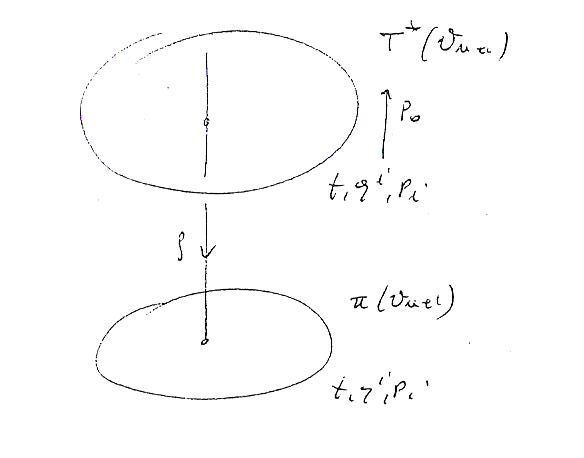
\includegraphics[width=0.5\columnwidth]{media/spazio-tempo-delle-fasi-e-struttura-di-poisson-di-tale-spazio/25-1.jpg}
\end{center}

$\pi (\mathcal{V}_{n+1})$ risulta essere una varietà differenziabile $2n+1$ dimensionale, riferita a coordinate \textit{naturali} $ t, q^i, P_i $, soggette alle leggi di trasformazione

\begin{equation*}
\begin{split}
& t' = t  \\
& q'^i = q'^i (t, q) \qquad q^i = q^i (t, q') \\
&P'_i = P_r \frac{\partial q^r}{\partial q'^i} \\
\end{split}
\end{equation*}

Una funzione $ f : \pi (\mathcal{V}_{n+1}) \rightarrow \mathbb{R} $ ($ f = f (t, q^i, P_i) $) dà luogo a una funzione $ f \circ \rho : T^* (\mathcal{V}_{n+1}) \rightarrow \mathbb{R} $ ($ f \circ \rho $ ancora descritta nella forma $ f = f (t, q^i, P_i) $). Viceversa, una funzione $ f $ definita sullo spazio $T^* (\mathcal{V}_{n+1}) $  può essere riguardata come il pull-back (attraverso $\rho$) di una funzione definita su $\pi(\mathcal{V}_{n+1})$, se e solo se $ f $ è costante lungo le fibre di $ \rho : T^* (\mathcal{V}_{n+1}) \rightarrow \pi (\mathcal{V}_{n+1}) $ ovvero se

\begin{equation} \label{eq:spazio-tempo_fasi_1}
\frac{\partial f}{\partial P_0} = 0 \qquad \Leftrightarrow \qquad \left\lbrace f, t \right\rbrace = 0
\end{equation}

si verifica facilmente che date due funzioni $ f, g $ costanti lungo le fibre di $ \rho : T^*(\mathcal{V}_{n+1}) \rightarrow \pi(\mathcal{V}_{n+1}) $, le loro parentesi di Poisson (ovviamente in $ T^* (\mathcal{V}_{n+1}) $) risulta indipendente da $ P_0 $: \\
infatti la condizione $\frac{\partial \left\lbrace f, g \right\rbrace }{\partial P_{0}} = 0$ equivale a $\left\lbrace \left\lbrace f, g \right\rbrace, t \right\rbrace = 0 $ (vedi ($ \ref{eq:spazio-tempo_fasi_1} $)) ma, per l'identità di Jacobi

\begin{equation}
\left\lbrace \left\lbrace f,g \right\rbrace ,t \right\rbrace = \left\lbrace f, \left\lbrace g,t \right\rbrace \right\rbrace - \left\lbrace g,\left\lbrace t,f \right\rbrace \right\rbrace 
\end{equation}
si ha che $ \left\lbrace g,t \right\rbrace=0$ e $\left\lbrace f,t \right\rbrace=0$ ($\Leftrightarrow \frac{\partial g}{\partial P_{0}} = 0 \text{ e } \frac{\partial f}{\partial P_{0}} = 0$) da cui la conclusione.\\
Pertanto è possibile definire operazione di \textit{parentesi di Poisson} in \textit{$\pi(\mathcal{V}_{n+1})$}
\begin{equation}
\left\lbrace f, g \right\rbrace = \frac{\partial f}{\partial q^i}\frac{\partial g}{\partial P_i}- \frac{\partial f}{\partial P_i}\frac{\partial f}{\partial q^i} \qquad \forall f, g \in \mathcal{F}(\pi (\mathcal{V}_{n+1}))
\end{equation}
Notare che $\pi (\mathcal{V}_{n+1})$ \textit{non} è una varietà simplettica (ad esempio perchè ha dimensione dispari), quindi l'esistenza di una parentesi di Poisson in $\pi (\mathcal{V}_{n+1})$ risulta un fatto non banale, e, come vedremo, molto importante.


\section{Trasformazione di Legendre vista più geometricamente}
\setcounter{equation}{0}

\begin{center}
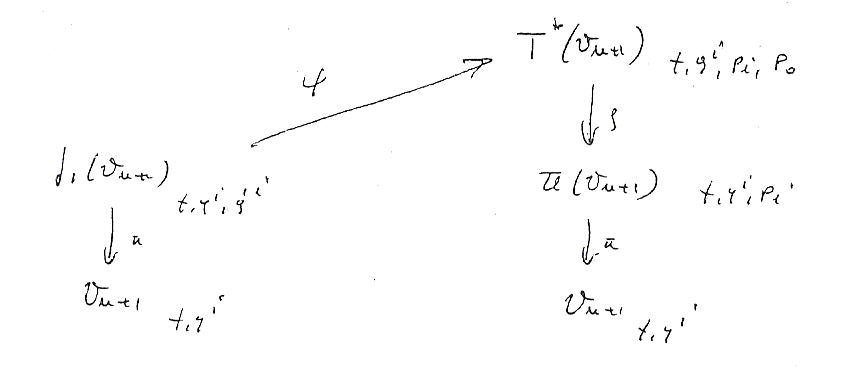
\includegraphics[width=\columnwidth]{media/trasformazione-di-legendre-vista-piu-geometricamente/26-1.jpg}
\end{center}

Vogliamo considerare una applicazione $ \psi : j_1 (\mathcal{V}_{n+1}) \longrightarrow T^* (\mathcal{V}_{n+1}) $. Dal punto di vista geometrico, essa vuole rappresentare una superficie di dimensione $ 2n+1 $ in $ T^* (\mathcal{V}_{n+1}) $, precisamente l'immagine $ \psi (j_1 (\mathcal{V}_{n+1})) $ in $ T^* (\mathcal{V}_{n+1}) $.

Richiediamo che $ \psi $ commuti con la proiezione $ \pi $, cioè preservi il punto in $ \mathcal{V}_{n+1} $. In coordinate, $ \psi $ sarà rappresentata nella forma
\begin{equation*}
\begin{split} 
	\psi : \quad &
\begin{cases}
	t = t \\
	q^i = q^i \\
	P_0 = P_0 (t, q^i, \dot{q}^i) \\
	P_i = P_i (t, q^i, \dot{q}^i) \\
\end{cases}
	\text{ ( $ \psi $ commuta con $ \pi $ ) }
\end{split}
\end{equation*}

Ricordiamo che, su $ j_1 (\mathcal{V}_{n+1}) $, (che, ricordiamo, rappresenta la totalità degli stati cinetici del sistema) dato un sistema dinamico Lagrangiano, abbiamo una funzione Lagrangiana $ \Lagr (t, q, \dot{q}) $ e una $ 1 $-forma di \textit{Poincaré-Cartan}
\begin{equation*}
	\theta_{\Lagr} = - H dt + \frac{\partial \Lagr}{\partial \dot{q}^i} dq^i \quad \qquad H = \frac{\partial \Lagr}{\partial \dot{q}^k} d\dot{q}^k - \Lagr
\end{equation*}

Su $ T^* (\mathcal{V}_{n+1}) $ abbiamo invece la $ 1 $-forma \textit{canonica di Liouville}
\begin{equation*}
	\theta = P_0 dt + P_i d \dot{q}^i
\end{equation*}

Sussiste il seguente risultato (trasformazione di Legendre): \\
Esiste un'unica $ \psi : j_1 (\mathcal{V}_{n+1}) \longrightarrow T^* (\mathcal{V}_{n+1}) $ fibrata in $ \mathcal{V}_{n+1} $ (cioè commutante con le proiezioni $ \pi :  j_1 (\mathcal{V}_{n+1}) \longrightarrow \mathcal{V}_{n+1} $  e $ \pi \cdot \rho : T^* (\mathcal{V}_{n+1}) \longrightarrow \mathcal{V}_{n+1} $ ) tale che
\begin{equation*}
	\theta_{\Lagr} = \psi^* (\theta)
\end{equation*}

In coordinate, questa condizione diventa
\begin{equation*}
\begin{cases}
	t = t \\
	q^i = q^i \\
	P_0 = - H (t, q^i, \dot{q}^i) \\
	P_i = \frac{\partial \Lagr}{\partial \dot{q}^i} (t, q^i, \dot{q}^i)
\end{cases}
	H = \frac{\partial \Lagr}{\partial \dot{q}^i} \dot{q}^i - \Lagr
\end{equation*}

\begin{center}
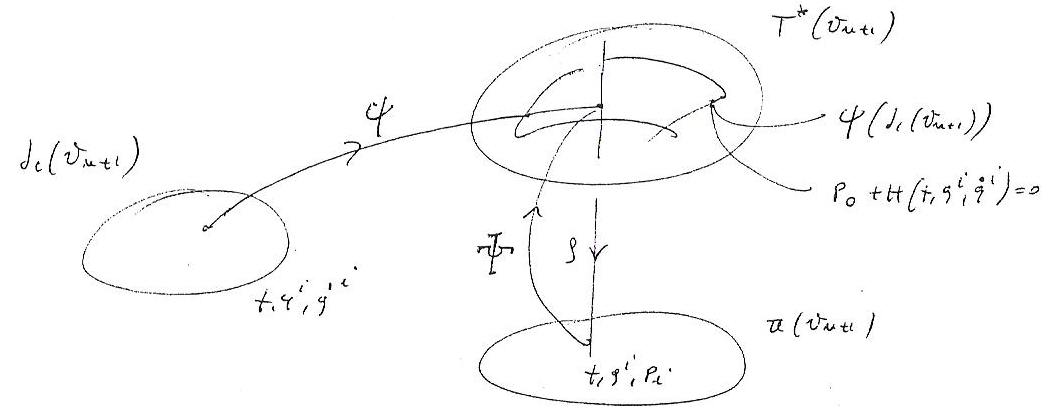
\includegraphics[width=\columnwidth]{media/trasformazione-di-legendre-vista-piu-geometricamente/26-2.jpg}
\end{center}

Ammesso, almeno localmente, che $ det \left( \frac{\partial^2 \Lagr}{\partial \dot{q}^i \partial \dot{q}^k} \right) \neq 0 $, la relazione $ P_i = \frac{\partial \Lagr}{\partial \dot{q}^i} (t, q^i, P_i) $ può essere posta nella forma
\begin{equation*}
	\dot{q}^i = \dot{q}^i (t, q^i, P_i)
\end{equation*}

e la funzione $ H $, definita inusualmente in funzione di $ t, q^i, \dot{q}^i $, può essere espressa in forma di $ t, q^i, P_i $:

% FINE PAGINA 26 - INIZIO PAGINA 27

\begin{equation*}
\begin{split}
H \left( t, q^i, P_i \right) &= \left( \frac{\partial \Lagr}{\partial \dot{q}^k} \dot{q}^k - \Lagr \right) \left( t, q^i, \dot{q}^i\left( t, q^i, P_i \right) \right) \\
&= \frac{\partial \Lagr}{\partial \dot{q}^k} \dot{q}^k \left( t, q^i, P_i \right) - \Lagr \left( t, q^i, \dot{q}^i\left( t, q^i, P_i \right) \right) \\
&= P_k \dot{q}^k \left( t, q^i, P_i \right) - \Lagr \left( t, q^i, \dot{q}^i \left( t, q^i, P_i \right) \right)
\end{split}
\end{equation*}

la superficie $ \Psi \left( j_1 (\mathcal{V}_{n + 1}) \right) $ può, a questo punto, essere espressa come luogo di zeri di

\begin{equation*}
P_0 + H \left( t, q^i, P_i \right) = 0
\end{equation*}

ovvero può essere rappresentata parametricamente nella forma

\begin{equation*}
t = t, \quad q^i = q^i, \quad P_i = P_i, \quad P_0 = - H \left( t, q^i, P_i \right)
\end{equation*}

come immagine attraverso $ \Psi $, di $ \pi(\mathcal{V}_{n + 1}) $.\\

La funzione $ H = H \left( t, q^i, P_i \right) $, riguardata come funzione di $ t, q^i, P_i $, è detta la \textit{funzione Hamiltoniana} del sistema (descritto dalla precedente Lagrangiana $ \Lagr $). \\

Con calcoli banali, abbiamo le ralazioni seguenti:

\begin{equation*}
\begin{split}
\frac{\partial H}{\partial P_r} = \dot{q}^r - \cancel{P_k \frac{\partial \dot{q}^k}{\partial P_r}} - \cancel{\frac{\partial \Lagr}{\partial \dot{q}^k} \frac{\partial \dot{q}^k}{\partial P_r}} = \dot{q}^r \\
\frac{\partial H}{\partial t} = \cancel{P_k \frac{\partial \dot{q}^k}{\partial t}} - \frac{\partial \Lagr}{\partial t} - \cancel{\frac{\partial \Lagr}{\partial t} \frac{\partial \dot{q}^k}{\partial t}} = - \frac{\partial \Lagr}{\partial t} \\
\frac{\partial H}{\partial q^i} = \cancel{P_k \frac{\partial \dot{q}^k}{\partial q^i}} - \frac{\partial \Lagr}{\partial q^i} - \cancel{\frac{\partial \Lagr}{\partial \dot{q}^k} \frac{\partial \dot{q}^k}{\partial q^i}} = - \frac{\partial \Lagr}{\partial q^i}
\end{split}
\end{equation*}

Infine, le equazioni di Lagrange

\begin{equation*}
\begin{cases}
\frac{dq^i}{dt} = \dot{q}^i \\
\frac{d}{dt} \frac{\partial \Lagr}{\partial \dot{q}^i} = \frac{\partial \Lagr}{\partial q^i}
\end{cases}
\end{equation*}

diventano, ponendo $ \frac{\partial \Lagr}{\partial \dot{q}^i} = P_i $

\begin{equation*}
\begin{cases}
\frac{dq^i}{dt} = \dot{q}^i \\
\frac{dP_i}{dt} = \frac{\partial \Lagr}{\partial q^i}
\end{cases}
\end{equation*}

e, per le relazioni dedotte sopra, %AAAAAAAAAAAAAAAAAAAAAAAAAAAAAAAAAAAAAAAAAA qui sarebbe utile inserire un ref

\begin{equation*}
\begin{cases}
\frac{dq^i}{dt} = \frac{\partial H}{\partial P_i} \\
\frac{dP_i}{dt} = - \frac{\partial H}{\partial q^i}
\end{cases}
\quad
H = H (t, q^i, P_i)
\end{equation*}

dette \textit{equazioni di Hamilton}, matematicamente equivalenti al campo

\begin{align*}
Z = \frac{\partial}{\partial t} + \frac{\partial H}{\partial P_i} \frac{\partial}{\partial q^i} - \frac{\partial H}{\partial q^i} \frac{\partial}{\partial P_i} \quad \text{ su } \pi(\mathcal{V}_{n + 1})
\end{align*}

Data una funzione $ f : \pi (\mathcal{V}_{n + 1}) \rightarrow \mathbb{R} $, $ f = f (t, q^i, P_i) $ l'evoluzione di $ f $ lungo i moti (cioè le curve in $ \pi(\mathcal{V}_{n + 1}) $ soluzioni delle equazioni di Hamilton) è data da

\begin{equation*}
\begin{split}
\frac{d}{d t} f &= \frac{\partial f}{\partial t} + \frac{\partial f}{\partial q^i} \frac{d q^i}{d t} + \frac{\partial f}{\partial P_i} \frac{d P_i}{d t} \\
&= \frac{\partial f}{\partial t} + \frac{\partial f}{\partial q^i} \frac{\partial H}{\partial P_i} - \frac{\partial f}{\partial P_i} \frac{\partial H}{\partial q^i} \\
&= \frac{\partial f}{\partial t} + \{ f, H \} \\
&= \{ f, P_0 \} + \{ f, H \}
\end{split}
\end{equation*}

% FINE PAGINA 27 - INIZIO PAGINA 28

con $ \{ f, H \} $ parentesi di Poisson in $ \pi(\mathcal{V}_{n + 1}) $ e $ \{ f, P_0 \} $ parentesi di Poisson in $ T^* (\mathcal{V}_{n+1}) $ (in $ \{ f, P_0 \} $, $ f $ viene riguardata ovviamente come funzione definita su $ T^* (\mathcal{V}_{n+1}) $, descitta ancora nella forma $ f = f (t, q^i, P_i) $). Riassumendo

\begin{equation*} \label{pag:trasf_leg_geom}
\frac{df}{dt} = \{ f, P_0 + H \} \qquad \qquad \longleftarrow \quad \text{parentesi di Poisson in $ T^* (\mathcal{V}_{n+1}) $}
\end{equation*}

In particolare, le equazioni di Hamilton diventano

\begin{equation*}
\begin{cases}
\frac{dq^i}{dt} = \{q^i, P_0 + H\} = \frac{\partial H}{\partial P_i} \\
\frac{dP_i}{dt} = \{P_i, P_0 + H\} = - \frac{\partial H}{\partial q^i}
\end{cases}
\end{equation*}

Infine

\begin{equation*}
\frac{dH}{dt} = \{H, P_0 + H\} = \{H, P_0\} = \frac{\partial H}{\partial t}
\end{equation*}

Facilmente si verificano i fatti seguenti:

\begin{itemize}
\item $ H $ non dipende esplicitamente dal tempo $ \Longrightarrow $ \, $ H $ integrale primo;
\item $ H $ non dipende esplicitamente da $ q^k $ $ \Longrightarrow $ \, $ P_k $ integrale primo;
\item $ f, g $ integrali primi $ \longrightarrow \{f, g\} $  integrale primo (conseguenza dell'identità di Jacobi).
\end{itemize}
\section{Trasformazioni canoniche sul cotangente e sullo spazio-tempo delle fasi}
Esaminiamo preliminarmente il problema nello spazio cotangente $ T^* (M) $, $ M $ essendo una varietà differenziabile di dimensione $ m $. Come abbiamo visto, riferito $ M $ a coordinate locali $ x^1, \dots , x^m $, è possibile riferire $ T^* (M) $ a coordinate $ x^1, \dots , x^m , y_1, \dots , y_m $, dette \textit{naturali}, sulla base dell'identificazione seguente

\begin{equation*}
\eta \in T^* (M) \Longleftrightarrow \eta = y_i (r) (dx^i)_{\pi (\eta)}
\end{equation*}

Una trasformazione tra $ 2 $ sistemi di coordinate \textit{naturali} è, come abbiamo già visto, del tipo

\begin{equation*}
\begin{cases}
x'^i = x'^i(x^1, \dots, x^m) \\
y'_i = y_r \frac{\partial x^r}{\partial x'^i} \qquad \qquad x^r = x^r (x'^1, \dots , x'^m)
\end{cases}
\end{equation*}
$ T^* (M) $ è dotato canonicamente di una struttura simplettica

\begin{equation*}
\Omega (X, Y) = X_i Y^i - X^i Y_i
\end{equation*}

dove

\begin{equation*}
\begin{cases}
X = X^i\frac{\partial}{\partial x^i} + X_i\frac{\partial}{\partial y_i} \\
Y = Y^i\frac{\partial}{\partial x^i} + Y_i\frac{\partial}{\partial y_i}
\end{cases}
\in T^* (M)
\end{equation*}

e che, per \textit{trasformazioni di coordinate naturali}, $ \Omega $ risulta invariante nella sua descrizione in coordinate, cioè

\begin{equation*}
\Omega (X, Y) =  X_i Y^i - X^i Y_i = X'_i Y'^i - X'^i Y'_i
\end{equation*}

% FINE PAGINA 28 - INIZIO PAGINA 29

Ciò che vedremo è che $\Omega$ \textit{risulta invariante in forma rispetto a un gruppo di trasformazioni più generale del gruppo delle trasformazioni tra coordinate naturali}.\\
Tale gruppo, che caratterizzeremo nelle pagine seguenti, sarà detto il gruppo delle \textit{trasformazioni canoniche}. \\

\textit{Definizioni equivalenti:}
%definizioni
\begin{definition}
Una trasformazione di coordinate in $ T^* (M) $

\begin{align*}
x'^i = x'^i (x^1, \dots , x^m, y_1, \dots , y_m) \\
y'^i = y'^i (x^1, \dots , x^m, y_1, \dots , y_m)
\end{align*}

è detta \textit{canonica} se la rappresentazione delle parentesi di Poisson in $ T^* (M) $ viene primata :
%FIXME
\begin{equation*}
\begin{array}{cc}
\begin{aligned}
\{ f, g \} &= \frac{\partial f}{\partial x^i} \frac{\partial g}{\partial y_i} - \frac{\partial f}{\partial y_i} \frac{\partial g}{\partial x^i} = \\
&= \frac{\partial f}{\partial x'^i} \frac{\partial g}{\partial y'_i} - \frac{\partial f}{\partial y'_i} \frac{\partial g}{\partial x'^i}
\end{aligned}
&
\mathcal{8} f, g \in \mathcal{F} ( T^*(M)) \\
\end{array}
\end{equation*}
(si è indicato con f, g le funzioni f, g espresse nei diversi sistemi di coordinate).
\end{definition}

\begin{definition}
Una trasformazione di coordinate in $ T^* (M) $ è detta \textit{canonica} se vengono primate le parentesi di Poisson fondamentali:
\begin{eqnarray*}
\{x'^i,x'^j\}=0 & \{y'_i,y'_j\}=0 & \{x'^i,y'_j\}=\delta^{i}_{j}
\end{eqnarray*}
\end{definition}

L'equivalenza tra le due definizioni segue dalla proprietà $ 4 $ di pagina $ \pageref{pag:assioma_funz_comp}$:

\begin{equation*}
\begin{split}
  \{f,g\}&= \frac{\partial f}{\partial x'^i}\{x'^i,g\}+\frac{\partial f}{\partial y'_i} \{y'_i,g\}  \\
&= \frac{\partial f}{\partial x'^i}\biggl(\{x'^i,x'^j\} \frac{\partial f}{\partial x'^j}+\{x'^i,y'_j\} \frac{\partial f}{\partial y'_j} \biggr) + \frac{\partial f}{\partial y'_i}\biggl(\{y'_i,x'^j\} \frac{\partial f}{\partial x'^j}+\{y'_i,y'_j\} \frac{\partial f}{\partial y'_j} \biggr)\\
\end{split}
\end{equation*}
La conclusione è ovvia.
\\
\\
Torniamo al problema della caratterizzazione delle trasformazioni canoniche in $ T^*(\mathcal{V}_{n+1}) $.\\
Osserviamo innanzitutto che le \textit{trasformazioni di scambio} del tipo \label{pag:trasf_scambio}

\begin{equation*}
\begin{split} 
&
\begin{cases}
x'^k = y'_k \\
y'_k = - x^k\\
\end{cases}
\text{per qualche } k \in \{1, \dots , m\} \\
e~~~~~~&
\begin{cases}
x'^r = x^r \\
y'_r = y_r\\
\end{cases}
\text{per $ r $ diverso dai $ k $ presi sopra} \\
\end{split}
\end{equation*}
sono canoniche.\\ 
A parte questi casi particolari (non banali e interessanti per l'interpretazione fisica ( $ P \rightarrow q, q \rightarrow -P $ )), la caratterizzazione delle trasformazioni canoniche in $ T^* (M) $, anzichè a partire dalla rappresentazione \textit{esplicita}

\begin{align*}
x'^i &= x'^i(x^1, \dots , x^m, y_1, \dots , y_m)
\\
y'_i &= y'_i(x^1, \dots , x^m, y_1, \dots , y_m)
\end{align*}

sarà svolta più agevolmente a partire dalla rappresentazione \textit{implicita}

\begin{align*}
x'^i &= x'^i(x^1, \dots , x^m, y'_1, \dots , y'_m)
\\
y_i &= y_i(x^1, \dots , x^m, y'_1, \dots , y'_m)
\end{align*}

% FINE PAGINA 29 - INIZIO PAGINA 30

il legame tra le due rappresentazioni, essendo garantito almeno localmente dal teorema della funzione implicita, ogni volta che sia valida la condizione

\begin{equation*}
det
\left( \frac{\partial (y_1, \dots, y_m)}{\partial (y'_1, \dots, y'_m)} \right)
\ne 0
\end{equation*}

(con $ x^1, \dots , x^m $ aventi un ruolo parametrico).
\\
\textit{Sussiste il seguente risultato:}\\
Condizione necessaria e sufficiente affinchè una trasformazione di coordinate in  $ T^* (M) $ data nella forma

\begin{align*}
x'^i &= x'^i(x,y')
\\
y_i &= y_i(x,y')
\end{align*}

sia \textit{canonica}, è che le funzioni $ x'^i $ , $ y_i $ sopra introdotte soddisfino le condizioni di \textit{irrotazionalità}

\begin{align*}
\frac{\partial x'^i}{\partial y'_j}=\frac{\partial x'^j}{\partial y'_i}, \qquad \frac{\partial x'^i}{\partial x^j}=\frac{\partial y_j}{\partial y'_i}, \qquad \frac{\partial y_i}{\partial x^j}=\frac{\partial y_j}{\partial x^i}.
\end{align*}
\\

Esprimiamo la trasformazione $ x^i, y_i \longleftrightarrow x'^i, y'_i $ nella forma

\begin{align*}
x'^i &= x'^i (x^1, \dots , x^m, y'_1, \dots , y'_m) = x'^i (x, y') \\
y_i &= y_i (x^1, \dots , x^m, y'_1, \dots , y'_m) = y_i (x, y')
\end{align*}

e caratterizziamo le trasformazioni tali che

\begin{equation*}
X'_i Y'^i - X'^i Y'_i = X_i Y^i - X^i Y_i
\end{equation*}

per ogni coppia di campi $ X, Y $. \\
La condizione suddetta equivale a:

\begin{equation*}
\begin{split}
&<dy'_i, X><dx'^i, Y>-<dx'^i, X><dy'_i, Y> =\\
&= <dy_i, X><dx^i, Y>-<dx^i, X><dy_i, Y>  \quad \qquad \forall X, Y
\end{split}
\end{equation*}
\\
\begin{equation*}
\begin{split}
&<dy'_i, X> <\frac{\partial x'^i}{\partial x^k} dx^k + \frac{\partial x'^i}{\partial y'_k}dy'_k, Y> - <\frac{\partial x'^i}{\partial x^k} dx^k + \frac{\partial x'^i}{\partial y'_k} dy'_k, X><dy'_i, Y> = \\
&= <\frac{\partial y_i}{\partial x^k} dx^k + \frac{\partial x'^i}{\partial y'_k} dy'_k, X><dx^i, Y> - <dx^i, X><\frac{\partial y_i}{\partial x^k} dx^k + \frac{\partial y_i}{\partial y'_k} dy'_k, Y> \quad \qquad \forall X, Y
\end{split}
\end{equation*}
\\

% FINE PAGINA 30 - INIZIO PAGINA 31

\begin{equation*}
\begin{split}
&\frac{\partial x'^i}{\partial x^k} <dy'_i \uline{, X>}<dx^k, Y> + \frac{\partial x'^i}{\partial y'_k} <dy'_i \uline{, X>}<dy'_k, Y> - \\
&\frac{\partial x'^i}{\partial x^k} <dx^k \uuline{, X>}<dy'_i, Y> - \frac{\partial x'^i}{\partial y'_k} <dy'_k \uline{, X>}<dy'_i, Y> = \\
&= \frac{\partial y_i}{\partial x^k}<dx^k \uwave{, X>}<dx^i, Y> + \frac{\partial y_i}{\partial y'_k}<dy'_k \uline{, X>}<dx^i, Y> - \\
& \frac{\partial y_i}{\partial x^k}<dx^i \uwave{, X>}<dx^k, Y> - \frac{\partial y_i}{\partial y'_k}<dx^i \uuline{, X>}<dy'_k, Y> \quad \qquad \forall X, Y
\end{split}
\end{equation*}

\begin{equation*}
\begin{split}
&\biggl(\frac{\partial x'^i}{\partial x^k} - \frac{\partial y_k}{\partial y'_i}\biggr)<dy'_i, X><dx^k, Y> + \biggl(\frac{\partial x'^i}{\partial y'_k} - \frac{\partial x'^k}{\partial y'_i} \biggr)<dy'_i, X><dy'_k, Y> - \\
&\biggl( \frac{\partial x'^i}{\partial x^k} - \frac{\partial y_k}{\partial y'_i} \biggr)<dx^k, X><dy'_i, Y> - \biggl(\frac{\partial y_i}{\partial x^k} - \frac{\partial y_k}{\partial x^i} \biggr)<dx^k, X><dx^i, Y> = 0
\end{split}
\end{equation*}
\\
e, per l'arbitrarietà
dei campi $ X, Y $, si ha
\begin{equation*}
\frac{\partial x'^i}{\partial x^k}-\frac{\partial y_k}{\partial y'_i}=0, \qquad \frac{\partial x'^i}{\partial y'_k}-\frac{\partial x'^k}{\partial y'_i}=0, \qquad \frac{\partial y_i}{\partial x^k}-\frac{\partial y_k}{\partial x^i}=0 \qquad i, k = 1, \dots , m
\end{equation*}

che possono essere riguardate come condizioni necessarie e localmente sufficienti per l'esistenza della rappresentazione \label{pag:trasf_can_pag24}

\begin{align*}
x'^i &= x'^i(x,y')=\frac{\partial F(x,y')}{\partial y'_i}
\\
y_i &= y_i(x,y')=\frac{\partial F(x,y')}{\partial x^i}
\end{align*}

della trasformazione di coordinate $ x^i, y_i \longleftrightarrow x'^i, y'_i $ in termini della funzione $F = F (x, y') = F (x^1, \dots , x^m, y'_1, \dots , y'_m) $, detta \textit{funzione generatrice} della trasformazione.\\
Ovviamente, assegnata una funzione $ F (x, y') $, essa definirà effettivamente una trasformazione se
\begin{equation*}
det
\left( \frac{\partial (y_1, \dots , y_m)}{\partial (y'_1, \dots , y'_m)} \right) = det \left( \frac{\partial^2  F}{\partial y'_i \partial x^j} \right) \ne 0
\end{equation*}

Notare che $ F $ risulta funzione delle \textit{vecchie} variabili $ x^1, \dots ,x^m $ e delle \textit{nuove} variabili $ y'_1, \dots ,y'_m $, e che quindi $ F $ definisce sempre una trasformazione canonica in modo \textit{implicito}.\\
Infine possiamo affermare che la \textit{più generale trasformazione canonica} si ottiene componendo una trasformazione canonica generata da $ F = F (x, y') $ nel modo sopra detto con trasformazioni di \textit{scambio} (vedi pagina \pageref{pag:trasf_scambio} ).


\section{Funzione generatrice}

\setcounter{equation}{0}

Torniamo ora a $\mathcal{V}_{n+1}$ e a $T^* (\mathcal{V}_{n+1})$. Le considerazioni precedenti si riportano a questo contesto restringendo l'attributo di \textit{canonico} ai sistemi di coordinate \\
\label{pag_funz_gen}
\begin{equation*}
	x^1, \dots ,x^m, y_1, \dots , y_n \equiv q^0, q^1, \dots , q^n, P_0, P_1, \dots , P_n
\end{equation*}
che, oltre a dare luogo alla \textit{rappresentazione} della $ 2 $-forma simplettica nella forma
\begin{equation*}
	\Omega(X, Y) = \sum_{\alpha = 0}^n \left( \langle dP_{\alpha}, X \rangle \langle dq^{\alpha}, Y \rangle - \langle dq^{\alpha}, X \rangle \langle dP_{\alpha}, Y \rangle \right)
\end{equation*}

\begin{equation*}
	\left( \iff \Omega(X, Y) = \sum_{\alpha = 0}^{n} X_{\alpha} Y^{\alpha} - X^{\alpha} Y_{\alpha} \right)
\end{equation*}

\begin{align*}
	X &= X^{\alpha} \frac{\partial}{\partial q^{\alpha}} + X_{\alpha} \frac{\partial}{\partial P_{\alpha}} \\
	Y &= Y^{\alpha} \frac{\partial}{\partial q^{\alpha}} + Y_{\alpha} \frac{\partial}{\partial P_{\alpha}}
\end{align*}
\textit{sussista l'identificazione} $q^o \equiv t$. \, $( t = \text{tempo} )$.

\begin{center}
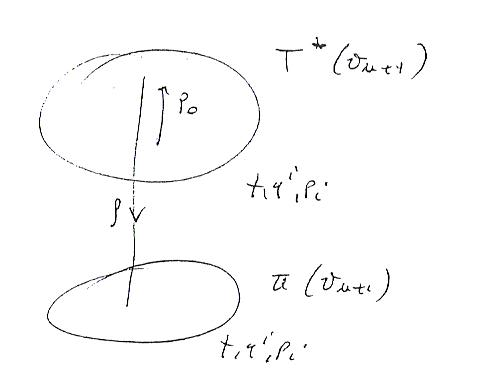
\includegraphics[width=0.5\columnwidth]{media/funzione-generatrice/32-1.jpg}
\end{center}

Le trasformazioni canoniche in $T^* (\mathcal{V}_{n+1})$ saranno quelle che preservano la rappresentazione della $2$-forma simplettica di $T^* (\mathcal{V}_{n+1})$ insieme all'identificazione $q^0 = t$ (cioè $q^{0'} = t' = t$ nelle nuove coordinate).

Avendo in mente la caratterizzazione delle trasformazioni canoniche data a pagina $\pageref{pag:trasf_can_pag24}$ in termini di una funzione generatrice, che ora chiamiamo $ \tilde{F} = \tilde{F} (t, q^1, \dots , q^n, P'_0, P'_1, \dots , P'_n) $, abbiamo
\begin{align*}
	q'^0 &= \frac{\partial \tilde{F}}{\partial P'_0} (t, q^1, \dots , q^n, P'_0, P'_1, \dots , P'_n) \\
	q'^i &= \frac{\partial \tilde{F}}{\partial P'_i} (t, q^1, \dots , q^n, P'_0, P'_1, \dots , P'_n) \\
	P_0 &= \frac{\partial \tilde{F}}{\partial t} (t, q^1, \dots , q^n, P'_0, P'_1, \dots , P'_n) \\
	P_i &= \frac{\partial \tilde{F}}{\partial q^i} (t, q^1, \dots , q^n, P'_0, P'_1, \dots , P'_n)
\end{align*}

Vediamo subito che la condizione $ q^{0'} = t' = t = q^0 $ implica
\begin{equation*}
	t' = \frac{\partial \tilde{F}}{\partial P'_0} = t
\end{equation*}
da cui
\begin{equation*}
	 \tilde{F} (t, q^1, \dots , q^n, P'_0, P'_1, \dots , P'_n) = P'_0 \cdot t + F (t, q^1, \dots , q^n, P'_0, P'_1, \dots , P'_n)
\end{equation*}
(da qui in avanti, dato l'uso frequente, chiameremo con $ F $ la parte di $ \tilde{F} $ depurata di $ P'_0 \cdot t $ (la $ F $ introdotta ora, evidentemente, \textit{non} è la $ F $ introdotta a pagina $ \pageref{pag:trasf_can_pag24} $ )).

Pertanto abbiamo
\begin{equation*}
\begin{cases}
	t' = t\\
	q'^i = \frac{\partial F}{\partial P'_i}\\
	P_0 = P'_0 + \frac{\partial F}{\partial t}\\
	P_i = \frac{\partial F}{\partial q^i}
\end{cases}
	F = F (t, q^1, \dots , q^n, P'_1, \dots , P'_n)
\end{equation*}
dove $ F = F (t, q^1, \dots , q^n, P'_1, \dots , P'_n) $

% FINE PAGINA 32 - INIZIO PAGINA 33

Le relazioni
\begin{align*}
	q'^i &= \frac{\partial F}{\partial P'_i} (t, q^i, P'_i)\\
	P_i &= \frac{\partial F}{\partial q^i} (t, q^i, P'_i)
\end{align*}
esprimono, in forma implicita (ma esplicitabile ogniqualvolta sia soddisfatta la condizione
\begin{equation*}
	det \left( \frac{\partial^2 F}{\partial q^i \partial P'_j} \right) \neq 0
\end{equation*}
che assicura l'applicabilità del teorema della funzione inversa) la trasformazione canonica generata da $ F (t, q^i, P'_i) $, mentre la relazione
\begin{equation*}
	P_0 = P'_0 + \frac{\partial F}{\partial t}
\end{equation*}
fornisce, indirettamente, la legge di trasformazione della funzione Hamiltoniana. Rappresentata la superficie $ \Psi (j_1 (\mathcal{V}_{n+1})) = \Psi (\pi (\mathcal{V}_{n+1})) \subset T^* (\mathcal{V}_{n+1}) $ nella forma
\begin{equation*}
	P_0 + H = P'_0 + H' = 0
\end{equation*}
si deduce
\begin{equation*}
	H' = H + \frac{\partial F}{\partial t}
\end{equation*}

(Ovviamente, affinché i due membri di quest'ultima relazione siano effettivamente confrontabili, occorre che il secondo membro (ad esempio) venga espresso in termini delle variabili del primo, $ t, q', P' $, utilizzando la trasformazione di coordinate generata da $ F $).

Riprendiamo la formula data a pagina $ \pageref{pag:trasf_leg_geom} $ che esprime l'evoluzione lungo i moti (cioè lungo le soluzioni delle equazioni di Hamilton) di una generica funzione $ f: \pi (\mathcal{V}_{n+1}) \longrightarrow \mathbb{R} $

\begin{equation*}
	\frac{df}{dt} = \{f, P_0 + H (t, q, P) \} = \{f, P'_0 + H' (t, q', P') \}
\end{equation*}

(Le parentesi di Poisson qui coinvolte sono ovviamente quelle in $ T^* (\mathcal{V}_{n+1}) $, e la $ f $ va pensata come il pull-back a $ T^* (\mathcal{V}_{n+1}) $ della $ f $ definita su $ \pi (\mathcal{V}_{n+1}) $).

\begin{equation*}
	\frac{df}{dt} = \{f, P'_0 \} + \{f, H' \} = \frac{df}{dt} + \frac{df}{dq'^i}\frac{dH'}{dP'_i} - \frac{df}{dP'_i}\frac{dH'}{dq'^i}
\end{equation*}
ovvero, in particolare, quando $ f = q'^i $ e $ f = P'_i $
\begin{align*}
	\frac{dq'^i}{dt} &= \frac{\partial H'}{\partial P'_i}\\
	\frac{dP'_i}{dt} &= - \frac{\partial H'}{\partial q'^i}
\end{align*}
ovvero, $ Z = \frac{\partial}{\partial t} + \frac{\partial H'}{\partial P'_i} \frac{\partial}{\partial q'^i} - \frac{\partial H'}{\partial q'^i} \frac{\partial}{\partial P_i} $
il che mostra \textit{l'invarianza in forma delle equazioni di Hamilton per effetto di una trasformazione canonica}.

\section{Teorema di Liouville sulla preservazione del \textit{volume} nello spazio delle fasi da parte della dinamica Hamiltoniana}

Consideriamo lo spazio-tempo delle fasi $ \pi (\mathcal{V}_{n+1}) $. Come abbiamo visto, esso risulta naturalmente fibrato su $ \mathcal{V}_{n+1} $. Ricordando che $ \mathcal{V}_{n+1} $ è \textit{fibrato su $ \mathbb{R} $} attraverso la proiezione al tempo assoluto $ t $, ne segue che $ \pi (\mathcal{V}_{n+1}) $ può essere riguardato come fibrato su $ \mathbb{R} $, attraverso una proiezione che continueremo a chiamare $ t $.

\begin{center}
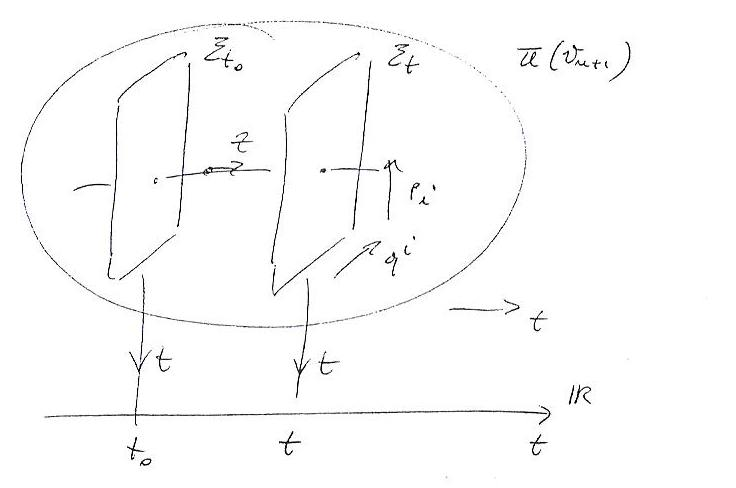
\includegraphics[width=0.65\columnwidth]{media/teorema-di-liuville-sulla-preservazione-del-volume-nello-spazio-delle-fasi-da-parte-della-dinamica-hamiltoniana/34-1.jpg}
\end{center}

indichiamo con $ \Sigma_t $ la fibra a t costante di $ t : \pi (\mathcal{V}_{n+1}) \longrightarrow \mathbb{R} $.
Evidentemente $ \Sigma_t $ costituisce una varietà differenziabile $ 2n $-dimensionale, riferibile a coordinate $ q^i, P_i$.
La dinamica Hamiltoniana, espressa dal campo vettoriale

\begin{equation*}
 Z = \frac{\partial}{\partial t} + \frac{\partial H}{\partial P_i} \frac{\partial}{\partial q^i} - \frac{\partial H}{\partial q^i} \frac{\partial}{\partial P_i}
\end{equation*}

ovvero, le curve integrali di $ Z $, stabiliscono un processo di \textit{identificazione} tra le fibre $ \Sigma_t $ a tempi diversi. In relazione al risultato (\textit{teorema di Liouville}) che vogliamo provare, risulta rilevante il fatto che le varietà $ \Sigma_t $ risultano essere dotate \textit{canonicamente di una struttura simplettica}, espressa in coordinate di $ \pi (\mathcal{V}_{n+1}) $ nella forma

\begin{equation*}
\omega = dP_i \wedge dq^i \quad \qquad \left( \sum_{i=1}^n \right) 
\end{equation*}

Da questo fatto segue che la $ 2n $-forma differenziale 

\begin{equation*}
\omega^n \stackrel{def}{=} dP_i \wedge \dots \wedge dP_n \wedge dq^1 \wedge \dots \wedge dq^n
\end{equation*}

fornisce una definizione \textit{canonica dell'elemento di volume in $ \Sigma_t $}, mediante il quale impostare un metodo \textit{intrinseco di integrazione}.

\begin{center}
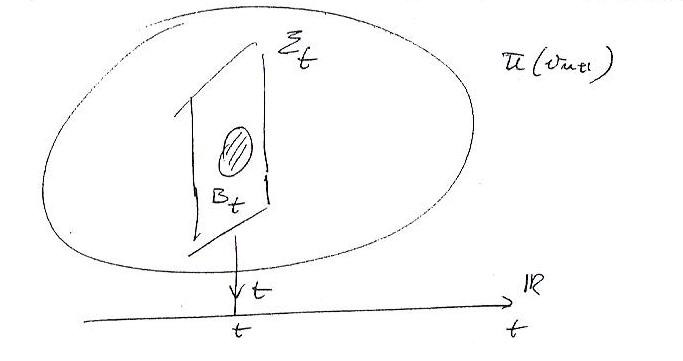
\includegraphics[width=0.5\columnwidth]{media/teorema-di-liuville-sulla-preservazione-del-volume-nello-spazio-delle-fasi-da-parte-della-dinamica-hamiltoniana/34-2.jpg}
\end{center}

Quanto detto consente di attribuire a un dominio integrabile ($ 2n $-dimensionale) $ B_t \subset \Sigma_t $ un volume

\begin{equation*}
Vol \, B_t = \int_{B_t} \omega^n = \int_{B_t} dP_i \, \dots \, dP_n \, dq^1 \, \dots \, dq^n
\end{equation*}

Ciò che è rilevante è \textit{l'intrinsecità} della valutazione data, ovvero l'indipendenza della stessa dalla scelta del sistema di coordinate.

% INIZIO PAGINA 35

Consideriamo nuovamente la dinamica \textit{Hamiltoniana} $ Z $.

\begin{center}
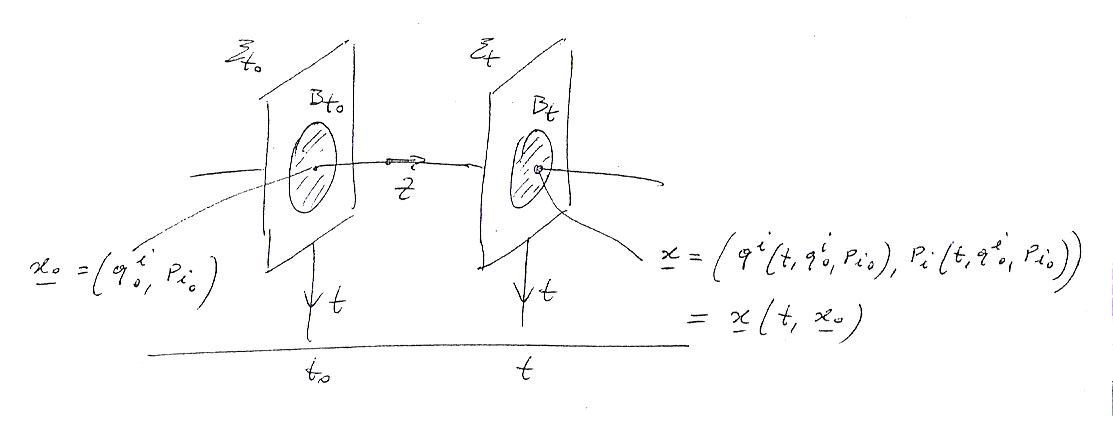
\includegraphics[width=0.95\columnwidth]{media/teorema-di-liuville-sulla-preservazione-del-volume-nello-spazio-delle-fasi-da-parte-della-dinamica-hamiltoniana/35-1.jpg}
\end{center}

Sia $ B_{t_0} $ un arbitrario dominio integrabile su $ \Sigma_{T_0} $ sia $ B_t $ ($ t $ arbitrario), il dominio che le curve integrali del vettore dinamico gli fanno corrispondere su $ \Sigma_t $.

Posto per semplicità di notazione

\begin{equation*}
\uline{x} = (\uline{P}, \uline{P}) = (q^1 \, \dots \, q^n, P_1 \, \dots \, P_n)
\end{equation*}

e indicato con

\begin{equation*}
\uline{x} = \uline{x} (t, \uline{x}_0)
\end{equation*}

le curve integrali (moti del sistema) di $ Z $, si ha

\begin{equation*}
Vol \, B_t  = \int_{B_t} dP_i \, \dots \, dP_n \, dq^1 \, \dots \, dq^n = \int_{B_t} (dx)^2n = \int_{B_{t_0}} \left| det \left( \frac{\partial \uline{x} (t, \uline{x}_0}{\partial \uline{x}_0} \right) \right| (dx_0)^{2n}
\end{equation*}

Notare che abbiamo ricondotto l'integrale nel dominio \textit{dipendente} dal tempo $ B_t $ all'integrale su un dominio \textit{fissato} $ B_0 $. Ovviamente l'integrando ora dipenderà da $ t $.
Ora, per questo fatto,

\begin{equation*}
\frac{d}{dt} Vol~B_t = \int_{B_{t_0}} \frac{\partial}{\partial t} \left| det \left( \frac{\partial \uline{x} (t, \uline{x}_0)}{\partial \uline{x}_0} \right) \right| (dx_0)^{2n}
\end{equation*}

Cominciamo a osservare che il segno di modulo è superfluo, essendo l'argomento dello stesso positivo,
Consideriamo nuovamente il campo dinamico

\begin{equation*}
 Z = \frac{\partial}{\partial t} + \frac{\partial H}{\partial P_i} \frac{\partial}{\partial q^i} - \frac{\partial H}{\partial q^i} \frac{\partial}{\partial P_i} = \frac{\partial}{\partial t} + X^i \frac{\partial}{\partial q^i} + X_i \frac{\partial}{\partial P_i}
\end{equation*}

dove

\begin{equation*}
X = X(t,\uline{x}) = \left( \frac{\partial H}{\partial P_1}, \dots ,\frac{\partial H}{\partial P_n}, \dots , -\frac{\partial H}{\partial q^1}, \dots , - \frac{\partial H}{\partial q^n} \right)
\end{equation*}

Sussiste il risultato seguente, di cui omettiamo per brevità la dimostrazione:

\begin{equation*}
\frac{\partial }{\partial t} det \left( \frac{\partial \uline{x} (t, \uline{x}_0}{\partial \uline{x}_0} \right) = \left( \sum_{\alpha = 1}^{2n} \frac{\partial X^\alpha}{\partial x^\alpha} \right) det \left( \frac{\partial \uline{x} (t, \uline{x}_0}{\partial \uline{x}_0} \right)
\end{equation*}

Osserviamo però che

\begin{equation*}
\begin{split}
\sum_{\alpha = 1}^{2n} \frac{\partial X^\alpha}{\partial x^\alpha} & = \sum_{k = 1}^{n} \frac{\partial X^k}{\partial q^k} + \sum_{k = 1}^{n} \frac{\partial X^{n+k}}{\partial P_k} = \\
& = \sum_{k = 1}^{n} \frac{\partial}{\partial q^k} \frac{\partial H}{\partial P_k} + \sum_{k = 1}^{n} \frac{\partial}{\partial P_k} \left( -\frac{\partial H}{\partial q^k}  \right) = 0
\end{split}
\end{equation*}

% INIZIO PAGINA 36

Collegando i passaggi so conclude che

\begin{equation*}
\frac{d}{dt} Vol \, B_t = 0
\end{equation*}

cioè che la dinamica Hamiltoniana preserva il volume di dominio arbitrario (integrabile) negli iperpiani $ \Sigma_t $. Questo risultato è noto come \textit{Teorema di Liouville}.



\end{document}
